\documentclass[12pt]{article}
% \usepackage{setspace}         % For line spacing if needed

\newcommand{\notebox}[1]{
\vspace{.5cm}
\hrule
\vspace{5pt}
{\Large \noindent \textit{Note :}\par}
   #1
\vspace{5pt}
\hrule
\vspace{.5cm} }

\newcommand{\figbox}[4]{
\begin{tcolorbox}[colback=cyan!5!white, colframe=white, boxrule=0mm, sharp corners] % 背景色等已经设置过
    \begin{center}
    \Large \textit{#1}
    \end{center}
    \vspace{.1cm}
   \begin{minipage}[t]{0.35\textwidth}  % 左侧放置图片的 minipage,并垂直居中
    \includegraphics[width=\linewidth, valign=t]{#2} % 用\includegraphics命令来放入图片文件
    \par  
    \vspace{20pt}
    \textit{#3} % 在图片下方放入注解文字
  \end{minipage}
  \hspace{0.03\textwidth}  % 水平间距
  \begin{minipage}[t]{0.62\textwidth}  % 右侧放置文本的 minipage
    {#4} %放入右侧文本
  \end{minipage}
\end{tcolorbox}
}
% adjust style for page
\usepackage{fancyhdr}
% adjust the gap between content and margins of pages 
\usepackage{geometry}
% import images
\usepackage{graphicx} 
% tweak math elements
\usepackage{amsmath}
% import other .tex files into the main .tex
\usepackage{import}
% for simulating model content
\usepackage{lipsum}
% for hyper link that connects to other URL
\usepackage{hyperref}
% for tables having specific width
\usepackage{tabularx} 
% together used with "tabularx" package
\usepackage{booktabs}
% control position of elements precisely
\usepackage{float}
% control the caption element for table and figure
\usepackage{caption}
% for some math symbols and format
\usepackage{amsmath} % for 'cases' environment
% To manage footnotes in tables
\usepackage{threeparttable}  
% i forget the function of this one, GPT told me to include it :) 
\usepackage{babel}
% for multirows
\usepackage{multirow}

% set the gap between the content and margins of page
\geometry{
top = 2.0cm,
bottom = 2cm,
left = 2.6cm,
right = 2.6cm
}




\title{Comparative Study of Time Series Models for Temperature Forecasting in Delhi}
\author{Feng Gu(T00751197), Yishu Liu(T00728937), Haoran He(T00749480)}
% \date{\today}

\begin{document}
\maketitle

\begin{center}
    \textbf{\large Abstract}
\end{center}

\sloppy
\textbf{
This study investigates regional temperature forecasting in Delhi, using climate data collected 
from 1st January 2013 to 24th April 2017. Various time series models, including dynamic regression 
model and linear regression, with and without dummy variables, alongside benchmark models like naive,
 drift, and mean forecasts were applied to the data. We evaluated the models’ performance using 
 metrics such as RMSE, MAE, and MAPE. Results indicate that the dynamic regression model with 
 SARIMA errors and dummy variables outperforms other models, achieving the lowest RMSE (3.0829)
and MAPE (12.4737). These findings highlight the effectiveness of incorporating dummy variables 
in improving temperature prediction accuracy, offering insights for future applications in climate
data modeling and decision-making}

% customized for showing github repo link
\textbf{
All associated code(including Latex) and files can be found in this \href{https://github.com/Gufeng-2002/Final-report-for-time-series.git}{GitHub repository}
\footnote{\href{https://github.com/Gufeng-2002/Final-report-for-time-series.git}{https://github.com/Gufeng-2002/Final-report-for-time-series.git}
}.
}




\section{Introduction}
\sloppy
The subject of global warming and climate change is gradually becoming one of the significant challenges 
that the world must face. More frequent and intense extreme weather events, such as heat waves, dust storms, 
and floods, have been observed globally \cite{dabhade2021}. 

The issue of climate change has become particularly crucial in large, densely populated cities. 
One such example is Delhi, India. The effects of climate change have intensified in recent years, 
posing challenges to human health, agricultural production, and the environment 
\cite{hussain2024}. 
Therefore, studying the temperature trends in Delhi holds high scientific value and practical significance. 
\sloppy
This study employs time series analysis, enabling the examination of historical temperature data,
comparison of different time series models, and the prediction of future temperature trends using the 
best-fit model. This research aims to provide a comprehensive understanding of temperature trends in the Delhi region,
and to explore and practice a more efficient way to organize and finish the paper writing work.

\section{Data}
\subsection{Source of data}
The climate data for the city of Delhi, India, spanning from 1st January 2013 to 24th April 2017, was downloaded 
from Kaggle\footnote{a machine learning community for learners} and originally sourced from 
Weather Undergroud API.  
The dataset consists 1576 records with date index and other 4 variables: mean temperature, 
humidity, wind speed and mean pressure. The mean temperature is the target variable and 
the other variables are used as predictors.


\subsection{Preparing and processing the data}
We process the raw data by following the procedure below:
\begin{itemize}
    \item We check the missing values in the training data and fill them using linear interpolation.
    \item We explore the distribution of the 4 variables, with boxplots and histogram shown in Figure 2 and 3. 
    Additionally, STL decomposition is applied to analyze the trend, seasonality and remainder of data, providing better understanding for the data.
    \item The abnormal outliers\footnote{outliers were detected using customized algorithm, which could be 
    found in the code of Module} 
    are replaced with corresponding moving average values.
    \item We create dummy variables from the "date" variable: four seasons. 
    \item Before the model fitting, we perform the stationary check and determine that the training data requires first-order differencing.   
\end{itemize}



\section{Method}
The complete code, latex documents and images can be found in the following \textbf{GitHub repo:}
\href{https://github.com/Gufeng-2002/Final-report-for-time-series.git}
{https://github.com/Gufeng-2002/Final-report-for-time-series.git}

\subsection{Specifing the desired model}
Before we set a specific model for forecasting \textit{meantemp}, 
we decomposed the \textit{meantemp} using TSL method\cite{fpp3stl}. Becasue
we have daily climate data, we set the season period as 365, assuming 
the same day in each year should have the most similar pattern in Temperature
\footnote{But it is not rigirous, because every 
four-year there is one more day premium and the number of day
is not an accurate "365" of interge.}.

After observing the possible seasonality and trend, we create a assume the model as following:
\[
y_t = \beta_{5 \times 1} X + \beta_{3 \times 1} H + \eta_t
\]
in which:
\[
X = \begin{bmatrix}
    1 & 1 & X_{11} & X_{21} & X_{31}\\
    1 & 2 & X_{12} & X_{22} & X_{32}\\
    & & ... & ... &\\
    1 & t & X_{1t} & X_{2t} & X_{3t} \\
    \end{bmatrix}
\quad H_i = 
\begin{bmatrix}
    1 & 0 & 0\\
    0 & 1 & 0\\
     & ... & \\
    0 & 0 & 0 \\
    \end{bmatrix} =
\begin{cases}
    1, \text{if the season is i} \\
    0, other wise
\end{cases}
\]
There are totally three $H_i$ here to aviod multilinearity 
caused by including intercept. To the $\eta_t$, we assume it follows
a SARIMA or ARIMA model, specificly:
\[
\Phi^P(B^s) \phi^p(B) (1-B^s)^D (1-B)^d \eta_t = 
\Theta^Q(B^s) \theta^q(B) \epsilon_t
\]
where, we set the $s$ equal to 365(days). The searching for peroper order  
of SARIMA((P,D,Q) and (p,d,q)) and the specific claculating are finished
by R language.

\subsection{Comparisions with other models}
In order to assess our model properly, we totally build \textbf{eight} models: Mean, Drift,
Naive, Snaive, Linear model with dummy variables or not, dynamic regression model with dummy variables or not
, shown in table 3, appendix.


\subsection{Complete workflow}

\subsubsection{ProcessRawData module of Python}
It is notable that the data processing steps are finished in a workflow with module \textit{"ProcessRawData.py"}
\cite{financialriskforecasting},
which has been pushed to the public Git repository. It can be easy
\footnote{only needing to point or change the directory path correctly} 
to repeat all these steps or make 
further adjustments to make it suitable for other work. 

\subsubsection{ModelFitting module of R}
To fit these models quickly and easily, we choose R to build these models and 
do relevant tests on them and visualize the results.
There is a \textit{"ModlFitting.R"} in the repo. There are
some functions that transport tables from R to Latex document, which 
accelerated our work.

\section{Results}
The specific settings about parameters of models can be found in the R module.

According the table 4 and 7, we compared the performance of these models on
training data and testing data, the dynamic regression model with dummy variables performs
well on training and testing data sets, its \textbf{RMSE(3.0829)} and \textbf{MAPE(12.4737)} are
the lowest in all models(standard linear regression with dummy variables of \textbf{RMSE(3.6619)} and \textbf{MAPE(13.7899)}).
The AICc and log\_lik are higher than linear models', but it is mainly becasue the 
number of parameters is more than models', which is reasonable.
Information about this model is shown in table 1.

From table 4 and 5 in appendix, we found that models with dummy variabes are always
better in performance than models without that. 
The four varialbes: \textit{time, season\_Autumn, season\_Spring, season\_Summer}
pass the 0.05 significance level test under the 
$H_{0}\footnote{$H_0$: the coefficient is value of 0, namely no influcence from this variable}$
assumption, however, they do not pass the corresponding tests in dynamic regression models.

To the reason why these variables become not important in dynamic regression,
one explanation might be that the influences from these four variables can be captured
well by the errors of SARIMA process in the model, and the long-term trend with \textit{time} is also
not imporant to mean temperature, based on the given sample.

Additionally, there is one counterintuitive coefficent: the coefficient
for \textit{season\_Summer} is smaller than that of \textit{season\_Spring}, which should 
not be correct by checking the summary about the average feature value in table 2(appendix).
It might indicate that some predictors in our model take the effect from \textit{season\_Summer},
if we remove these interfering factors, the relationship might be shown correctly, or this is 
the truth of the real word.

Although some coefficients did not pass the significance level test, we can still
use the model to forecast, becasue we are focusing on the relationship between these
variables but the future values of target. 

\begin{table}[!h]
    \centering
    \captionsetup{font=small} % Set caption to left-align and smaller font
    \caption{\textit{Summay about the dynamic regression model.
    Including the coefficents, tests about residuals from training data,
    and criteria about performance from testing data.
    (Note: the dynamic regression model here is called 'sarima\_dummy' in R code
     and tables in appendix)}}
    \label{tab:model_summary_combined}
    \begin{tabular}{lccccc}
    \toprule
    \textbf{Metric} & \textbf{ME} & \textbf{RMSE} & \textbf{MAE} & \textbf{MPE} \\
    \midrule
    \multirow{2}{*}{dynamic regression}
        & 0.5447 & 3.0829 & 2.6184 & -0.079 \\
        \cmidrule{2-5}
        & \textbf{MAPE} & \textbf{ACF1} & \textbf{log\_lik} & \textbf{AIC} \\
    \cmidrule{2-5}
        & 12.4737 & 0.8543 & -2369.349 & 4762.699 \\
    \midrule
    \textbf{Coefficient} & \textbf{Estimate} & \textbf{Std. Error} & \textbf{Statistic} & \textbf{P-value} \\
    \cmidrule{1-5}
    ar1            & 0.9898  & 0.0041 & 242.1087 & 0.0000 \\
    ma1            & -0.0953 & 0.0298 & -3.2015  & 0.0014 \\
    ma2            & -0.1798 & 0.0300 & -5.9982  & 0.0000 \\
    humidity       & -0.1363 & 0.0042 & -32.4098 & 0.0000 \\
    wind\_speed    & -0.0291 & 0.0072 & -4.0637  & 0.0001 \\
    meanpressure   & -0.0322 & 0.0076 & -4.2461  & 0.0000 \\
    time           & 0.0021  & 0.0045 & 0.4730   & 0.6363 \\
    season\_Autumn & 0.2608  & 0.5227 & 0.4990   & 0.6179 \\
    season\_Spring & 0.5930  & 0.5235 & 1.1326   & 0.2576 \\
    season\_Summer & 0.4116  & 0.6098 & 0.6751   & 0.4997 \\
    intercept      & 63.9278 & 8.5701 & 7.4594   & 0.0000 \\
    \midrule
    \textbf{Other Metrics} & \textbf{sigma2} & \textbf{log\_lik} & \textbf{AICc} & \textbf{BIC} \\
    \cmidrule{1-5}
    \multirow{2}{*}{dynamic regression} & 1.5048 & -2369.349 & 4762.914 & 4826.149  \\
    \cmidrule{2-5}
     & \textbf{lb\_stat} & \textbf{lb\_pvalue} & \textbf{bp\_stat} & \textbf{bp\_pvalue} \\
     \cmidrule{2-5}
     & 1.5524 & 0.2128 & 1.5492 & 0.2133 \\
    \bottomrule
    \end{tabular}
\end{table}

We also visualized the forecasts for all models to 
make the comparisons more clear and direct in figure 1.
\begin{figure}[!h]
    \centering
    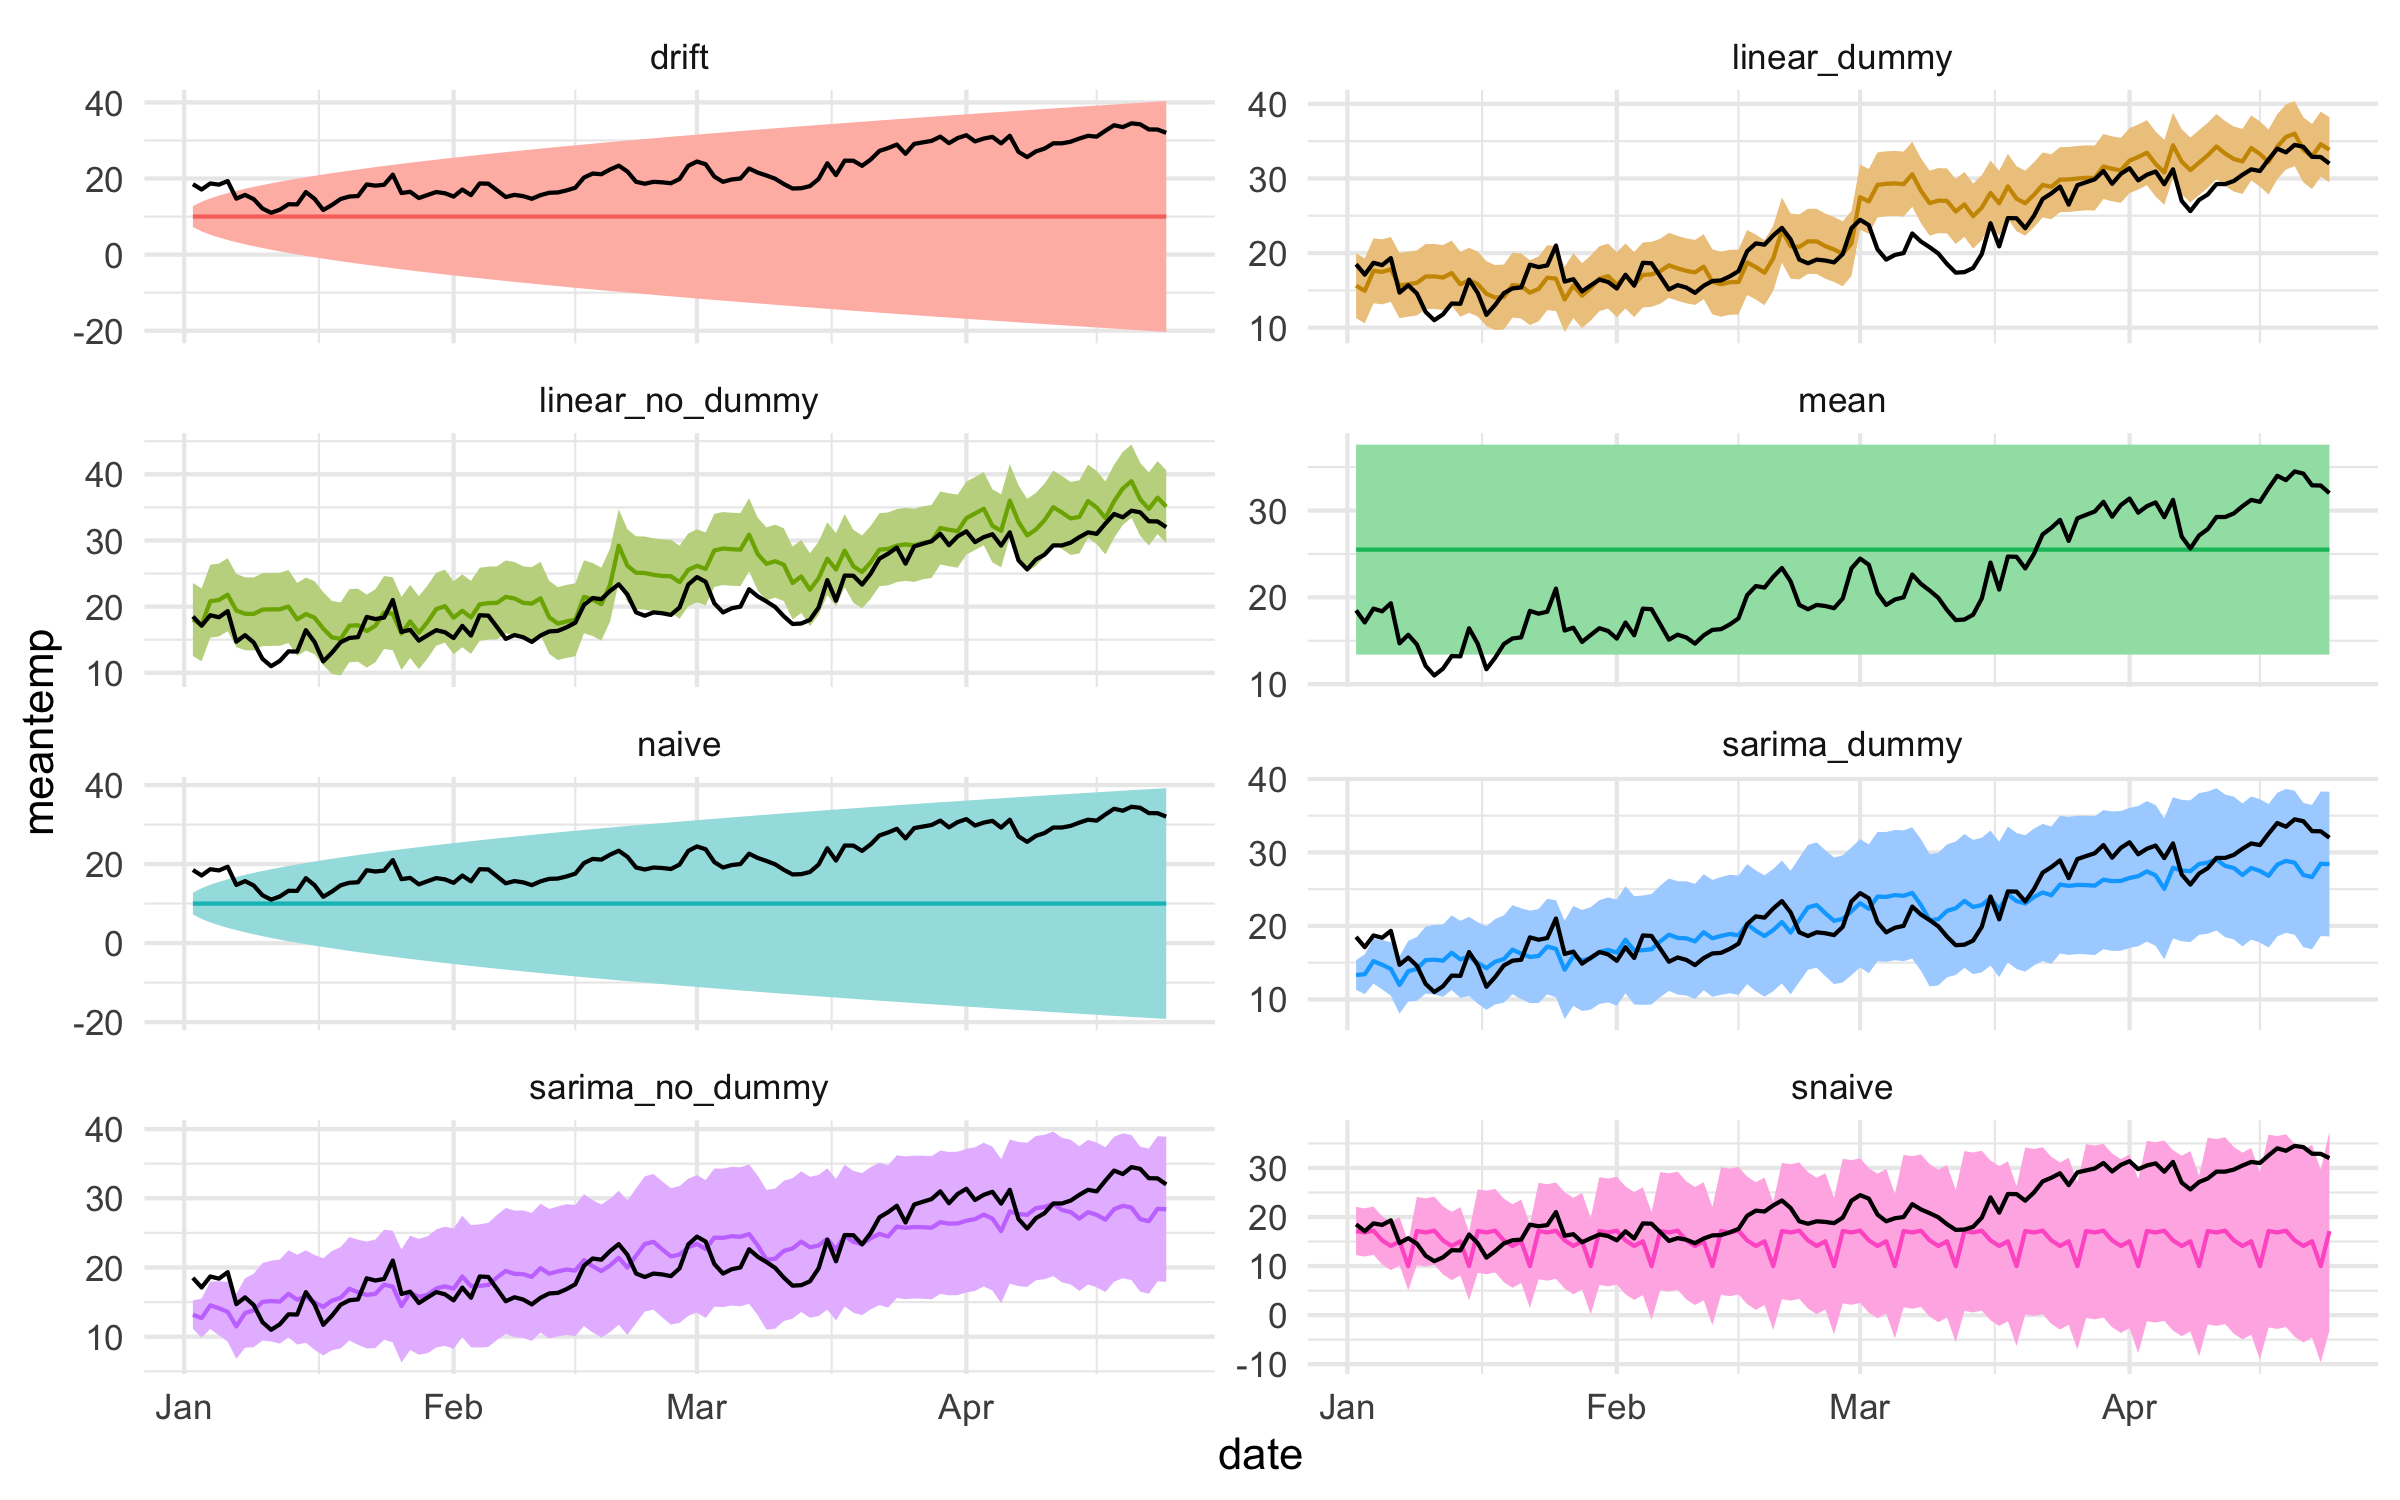
\includegraphics[width=.8\textwidth]{images/forecasts_CI90.png}
    \captionsetup{font=small} % Set caption to left-align and smaller font
    \caption{\textit{Forecasts from eight models. 
    Becasue of the assumptions and settings to models,
    we should compare the closes forecasts from dynamic regression model with forecasts
    from other models.}}
    \label{fig:figure1}
\end{figure}

\section{Discussion}
\subsection{Explanation about the model results}
According the regression results, we found that \textit{humidity, wind speed and mean pressure} have
negative effect on mean temperature, with their increases, the temperature decreases.
In comparison with the winter, the other seasons have higher mean temperature, 
even thought the coefficent of \textit{Spring} and \textit{Summer} might look counterintuitive, 
which could be the task for further exploration.

The autoregression and moving average parts show there are strong autocorrelation
in the mean temperature variable, which could be explained by standard linear model
that considers \textit{time and seasons} variables in some extent.

\subsection{Other useful work and further improvement.}
We have to admit it is not a very rigirous report due to the lack of time and 
the limits of our skills and professional knowledge in coding and Time Series field.

However, this report is a try in using Vscode, Rstudio, Latex entention as a complete
workflow, in which we manage to finish all the work in one system and make the
whole process automatic as much as possible. The complete frame work could be found in the GitHub
repository, including the document frame of Latex.

To make the whole workflow better, i think we can make improvement with the following
aspects:
\begin{itemize}
    \item Learn Time Series forecasting models more
    \item Be familiar with R and Python for Data Science
    \item Be familiar with using Vscode, Rstudio and GitHub for collaboration.
\end{itemize}

\clearpage
% Bibliography section
\begin{thebibliography}{99} % The number specifies the width of the label

    \bibitem{dabhade2021} 
    A. Dabhade, S. Roy, M. S. Moustafa, S. A. Mohamed, R. El Gendy, and S. Barma, 
    ``Extreme Weather Event (Cyclone) Detection in India Using Advanced Deep Learning Techniques,'' 
    \textit{2021 9th International Conference on Orange Technology (ICOT)}, 
    Tainan, Taiwan, 2021, pp. 1--4, 
    doi: \href{https://doi.org/10.1109/ICOT54518.2021.9680663}{10.1109/ICOT54518.2021.9680663}.

    \bibitem{hussain2024} 
    Hussain S., Hussain E., Saxena P., Sharma A., Thathola P., Sonwani S., 
    ``Navigating the impact of climate change in India: a perspective on climate action (SDG13) and sustainable cities and communities (SDG11),'' 
    \textit{Frontiers in Sustainable Cities}, 2024 Jan 23. 
    Available from: 
    \href{https://research-ebsco-com.ezproxy.tru.ca/linkprocessor/plink?id=6c6991da-78bd-3062-a586-5a5d83ba7467}{https://research-ebsco-com.ezproxy.tru.ca}.

    \bibitem{financialriskforecasting}
    A. McNeil. 
    ``Financial Risk Forecasting: R Best Practice,'' 
    \textit{Financial Risk Forecasting Notebook}. 
    Available at: \url{https://www.financialriskforecasting.com/notebook/R/BestPractice.html}. 
    Accessed: November 30, 2024.

    \bibitem{fpp3stl}
    H. Hyndman and G. Athanasopoulos. 
    ``STL Decomposition,'' 
    \textit{Forecasting: Principles and Practice (3rd ed.)}. 
    Available at: \url{https://otexts.com/fpp3/stl.html}. 
    Accessed: November 30, 2024.

\end{thebibliography}





\clearpage
\section{Appendix}

\subsection{Figures}

\begin{figure}[!h]
    \centering
    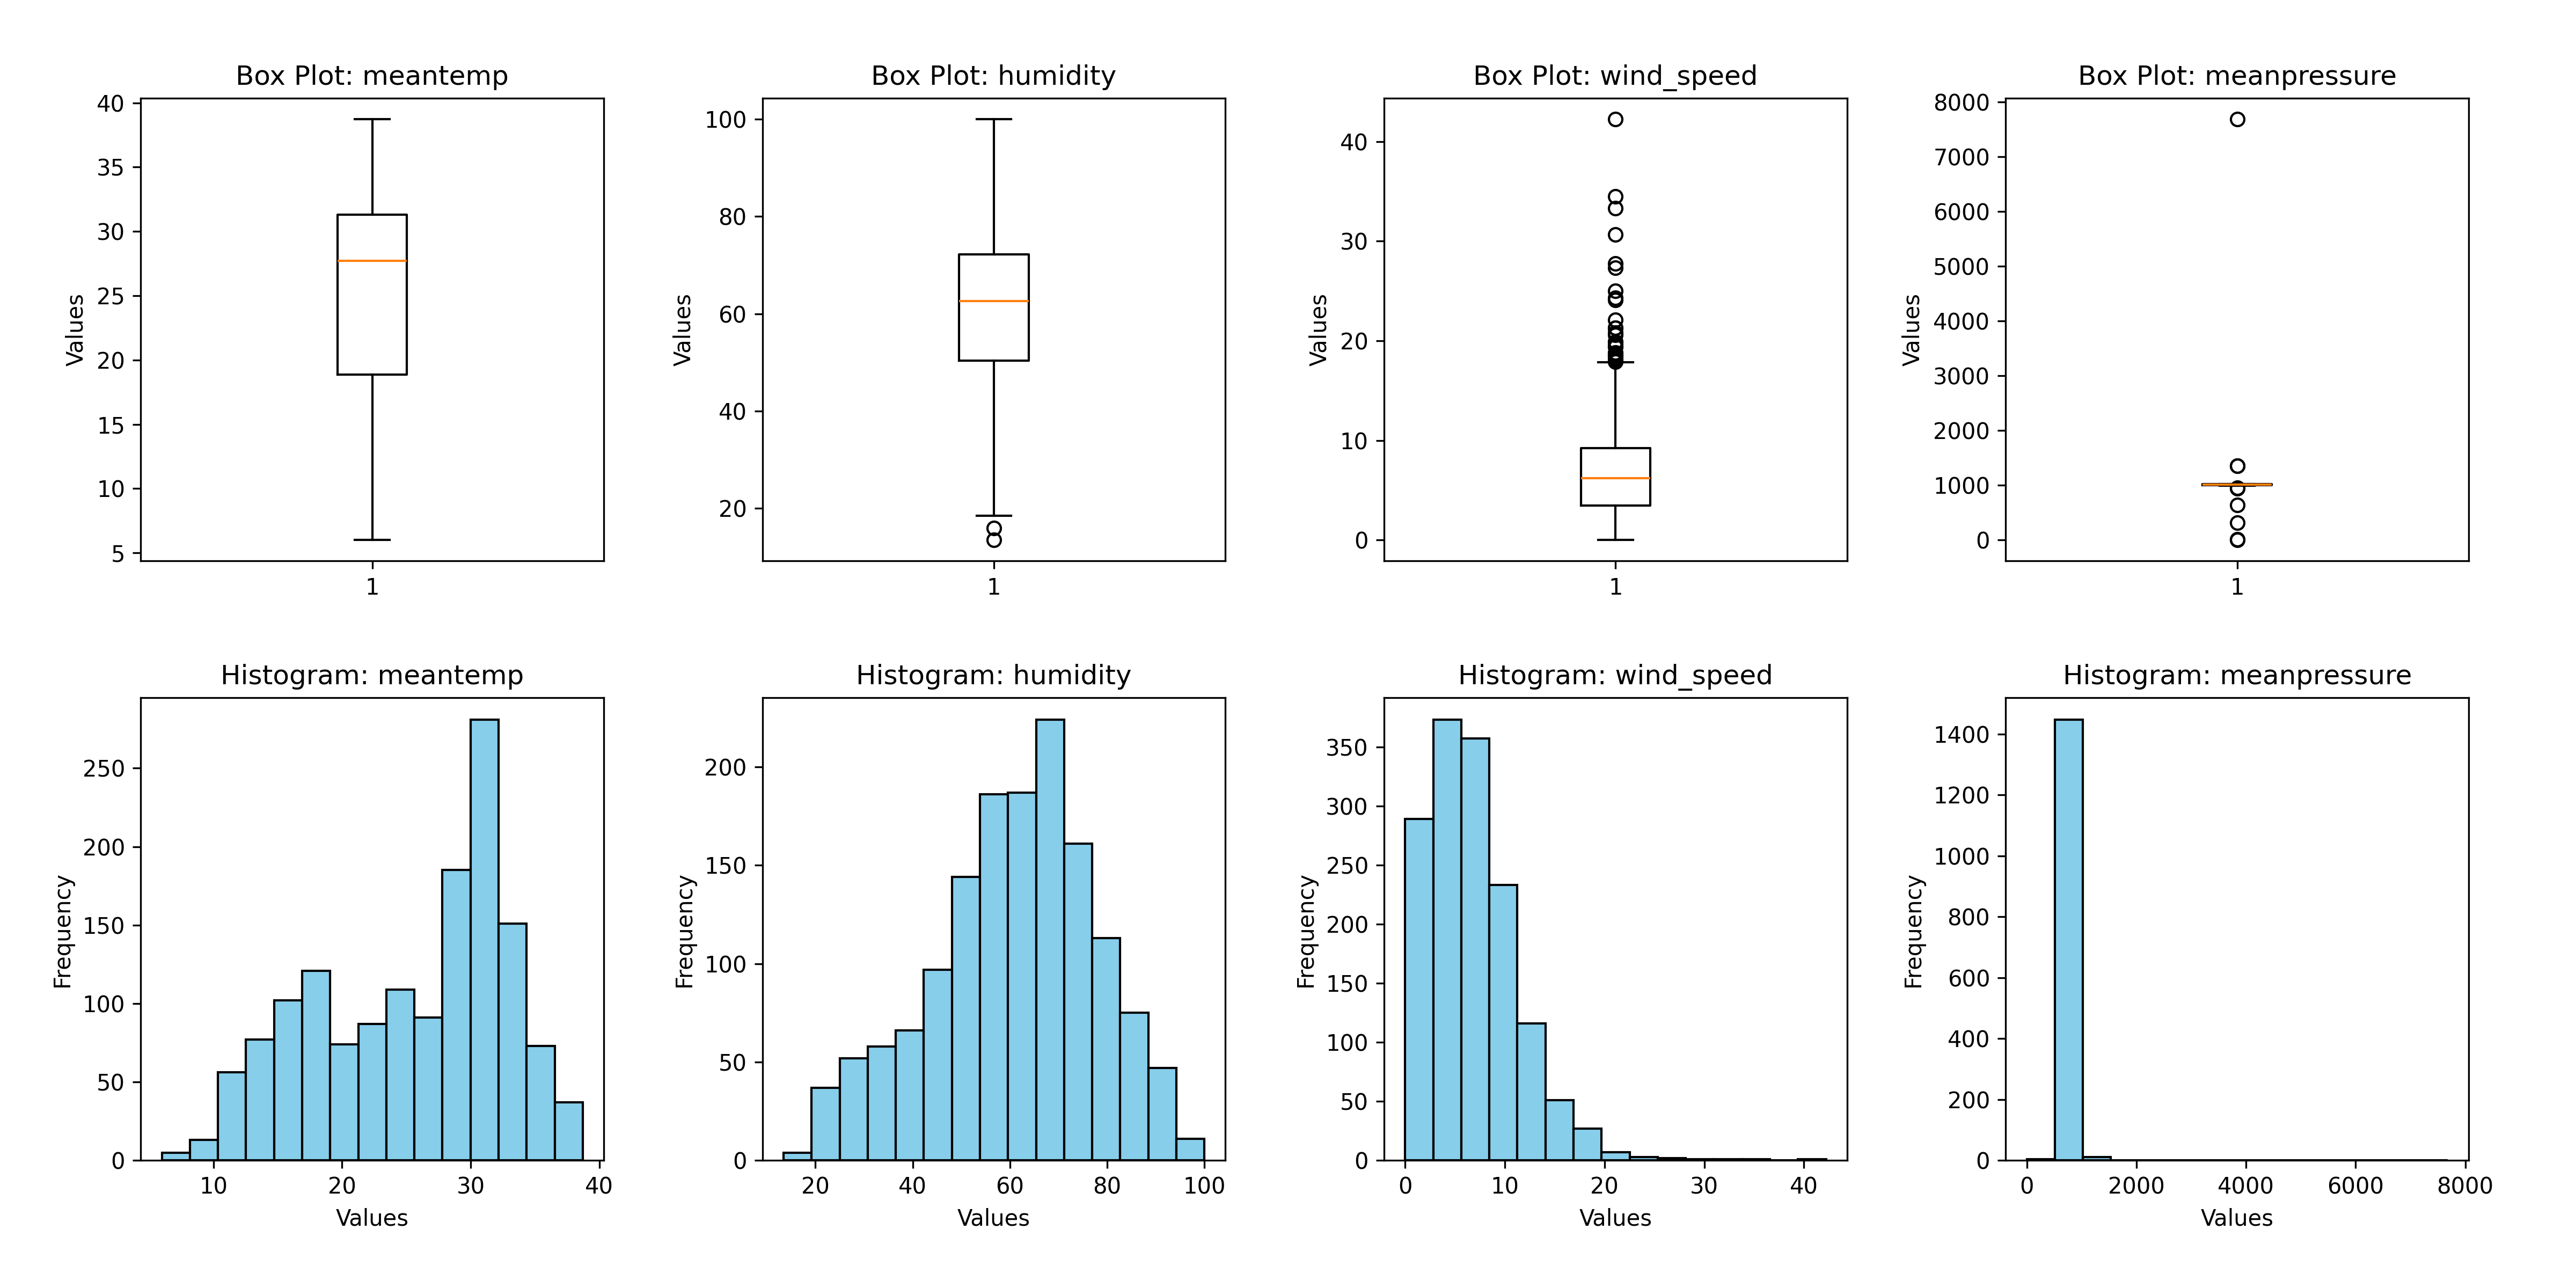
\includegraphics[width=.8\textwidth]{images/raw_train_data.png}
    \caption{\small \textit{Distribution of the raw data without replacing outliers}}
    \label{fig:figure1}
\end{figure}

\begin{figure}[!h]
    \centering
    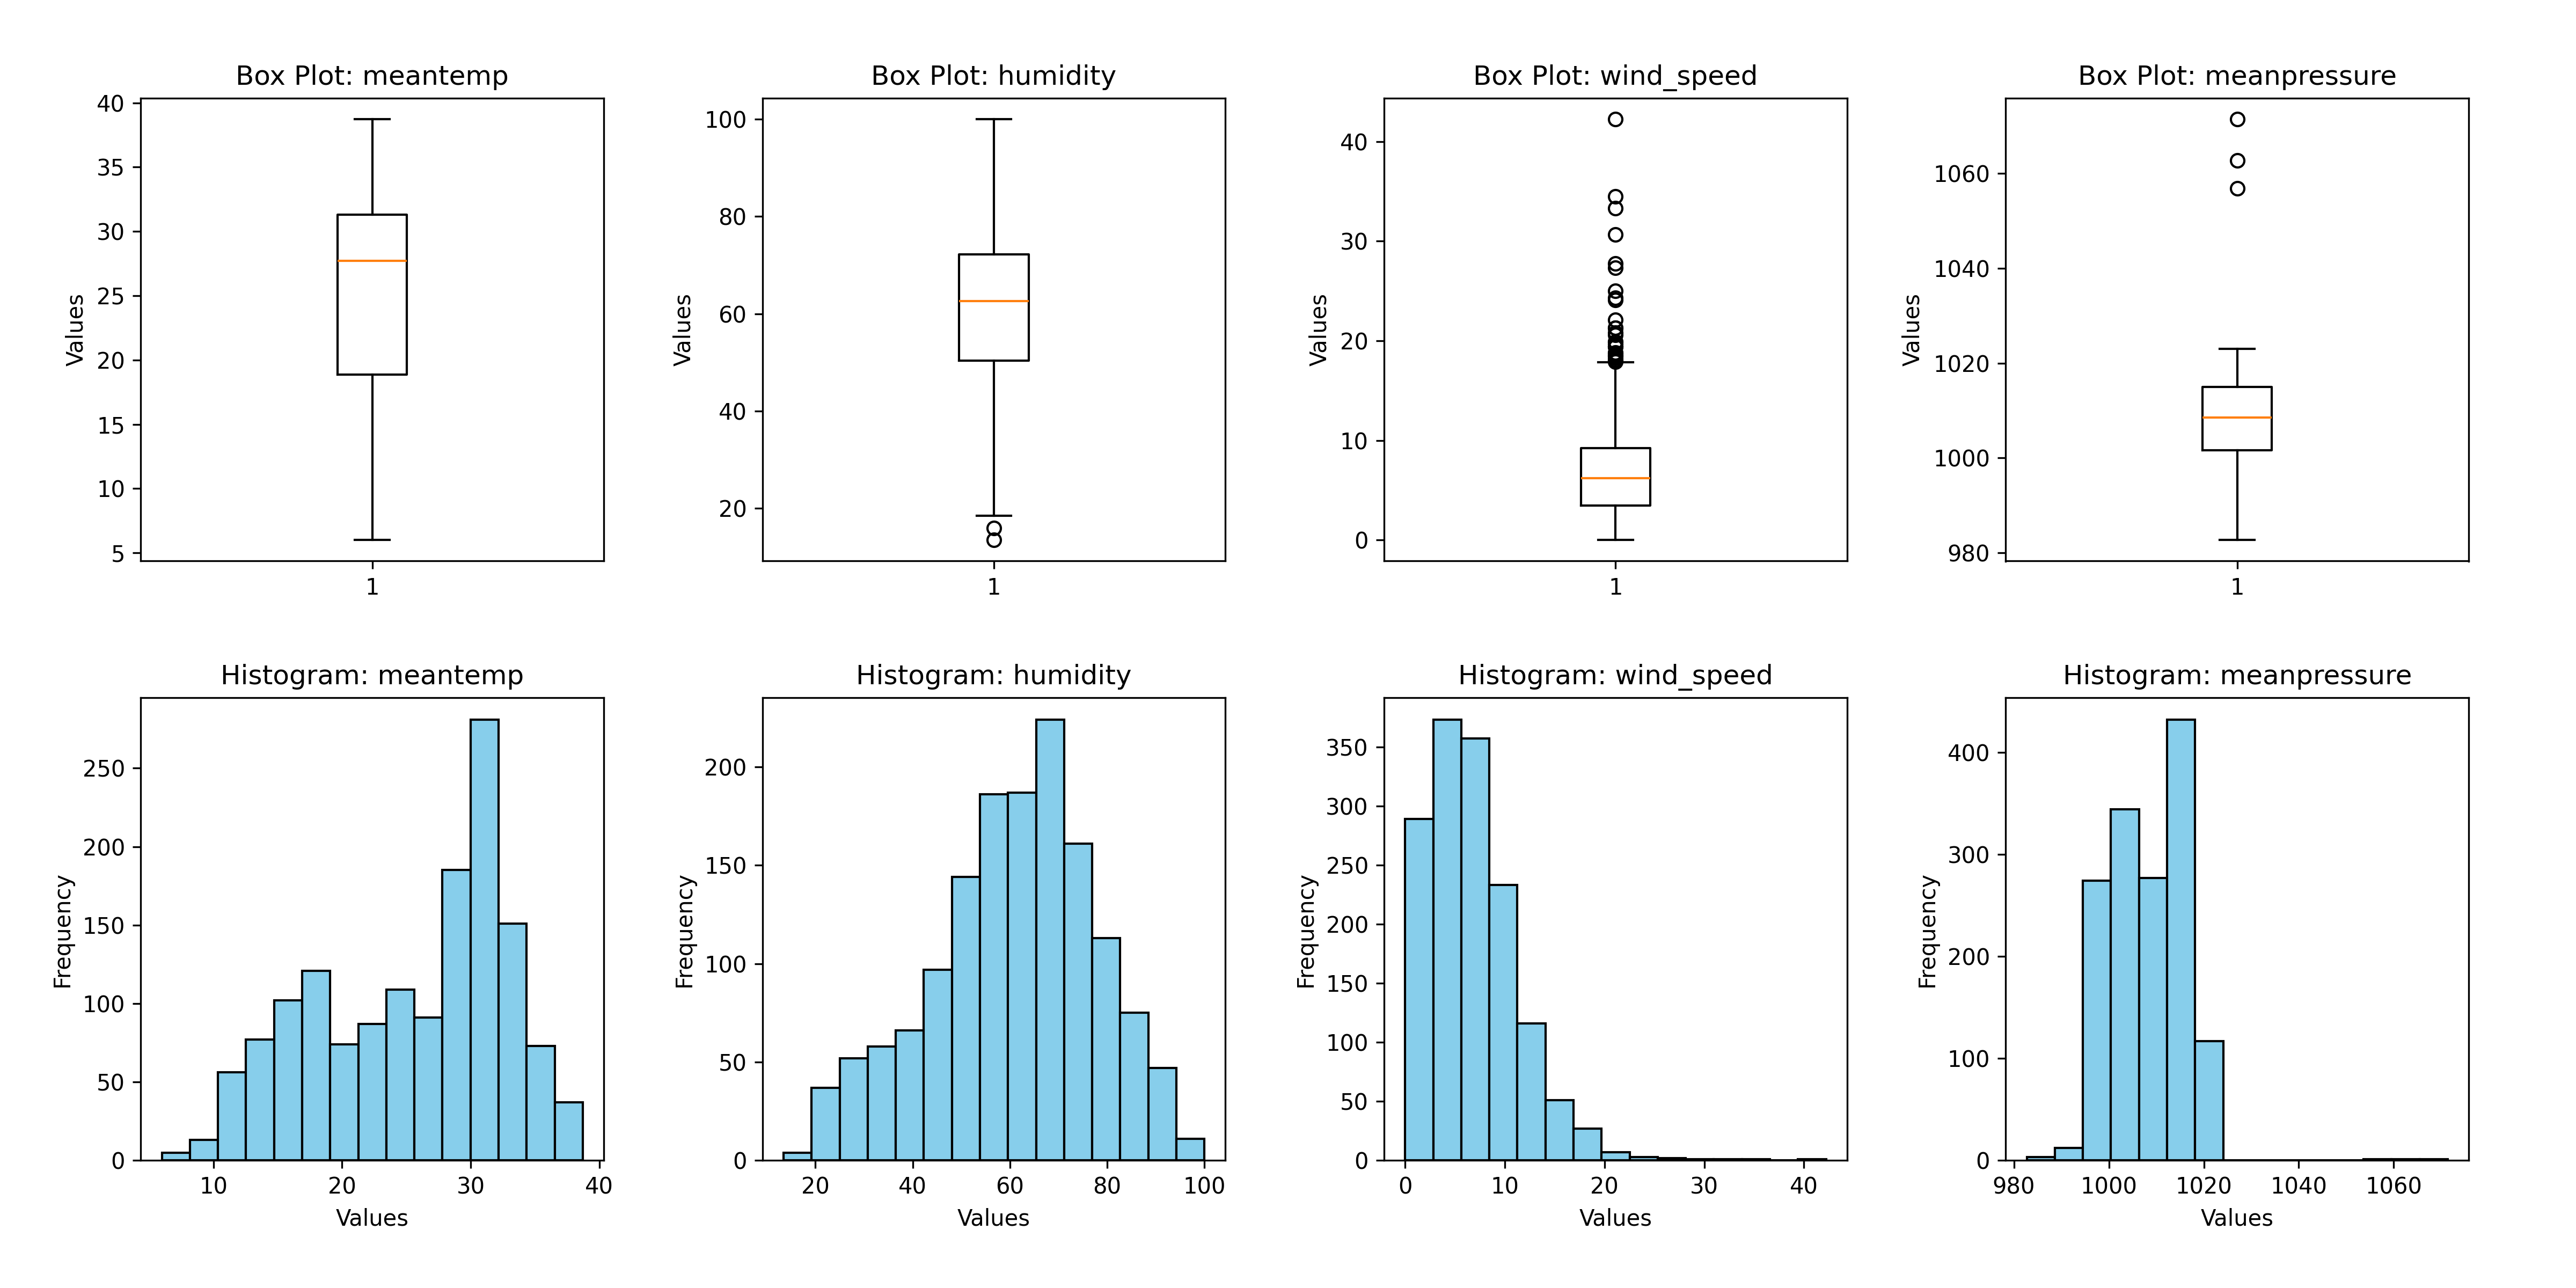
\includegraphics[width=.8\textwidth]{images/processed_train_data_box_and_hist_plots.png}
    \caption{\small \textit{Distribution of the processed data after replacing outliers}}
    \label{fig:figure1}
\end{figure}

\begin{figure}[!h]
    \centering
    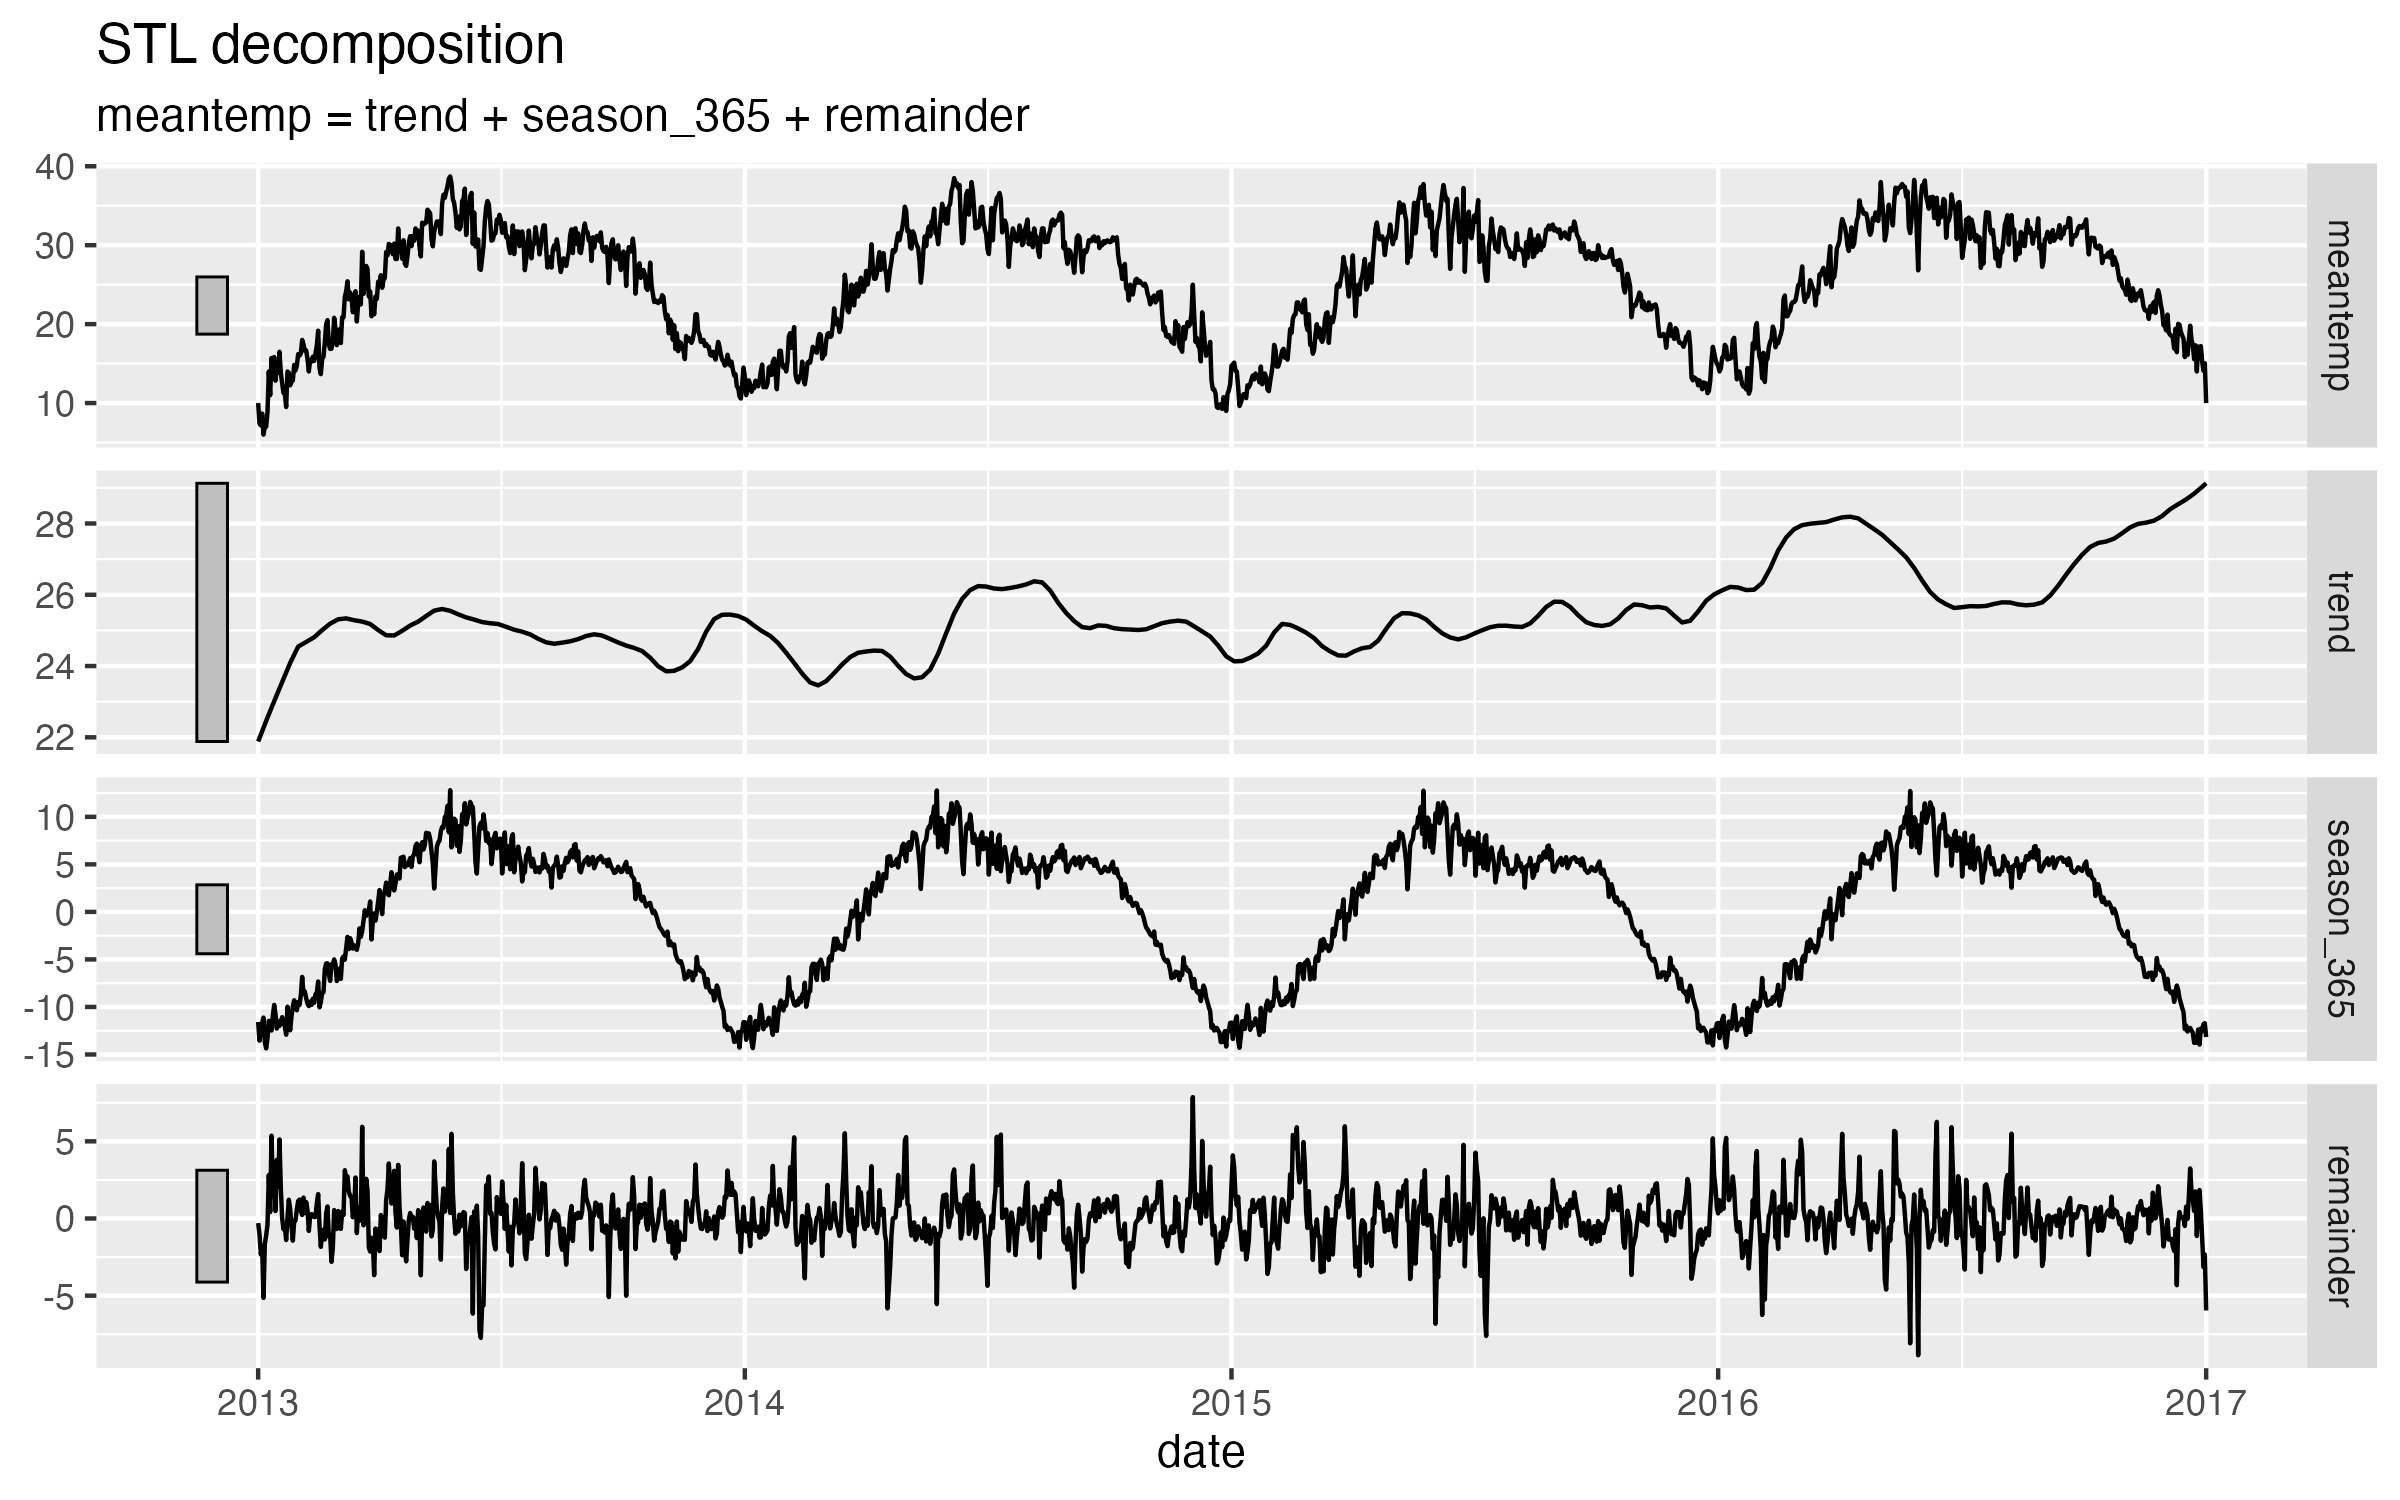
\includegraphics[width=.8\textwidth]{images/decomposition_plot.png}
    \caption{\small \textit{STL Decomposition of the mean temperature variable 
    (pointing period = 365 days)}}
    \label{fig:figure1}
\end{figure}

\begin{figure}[!h]
    \centering
    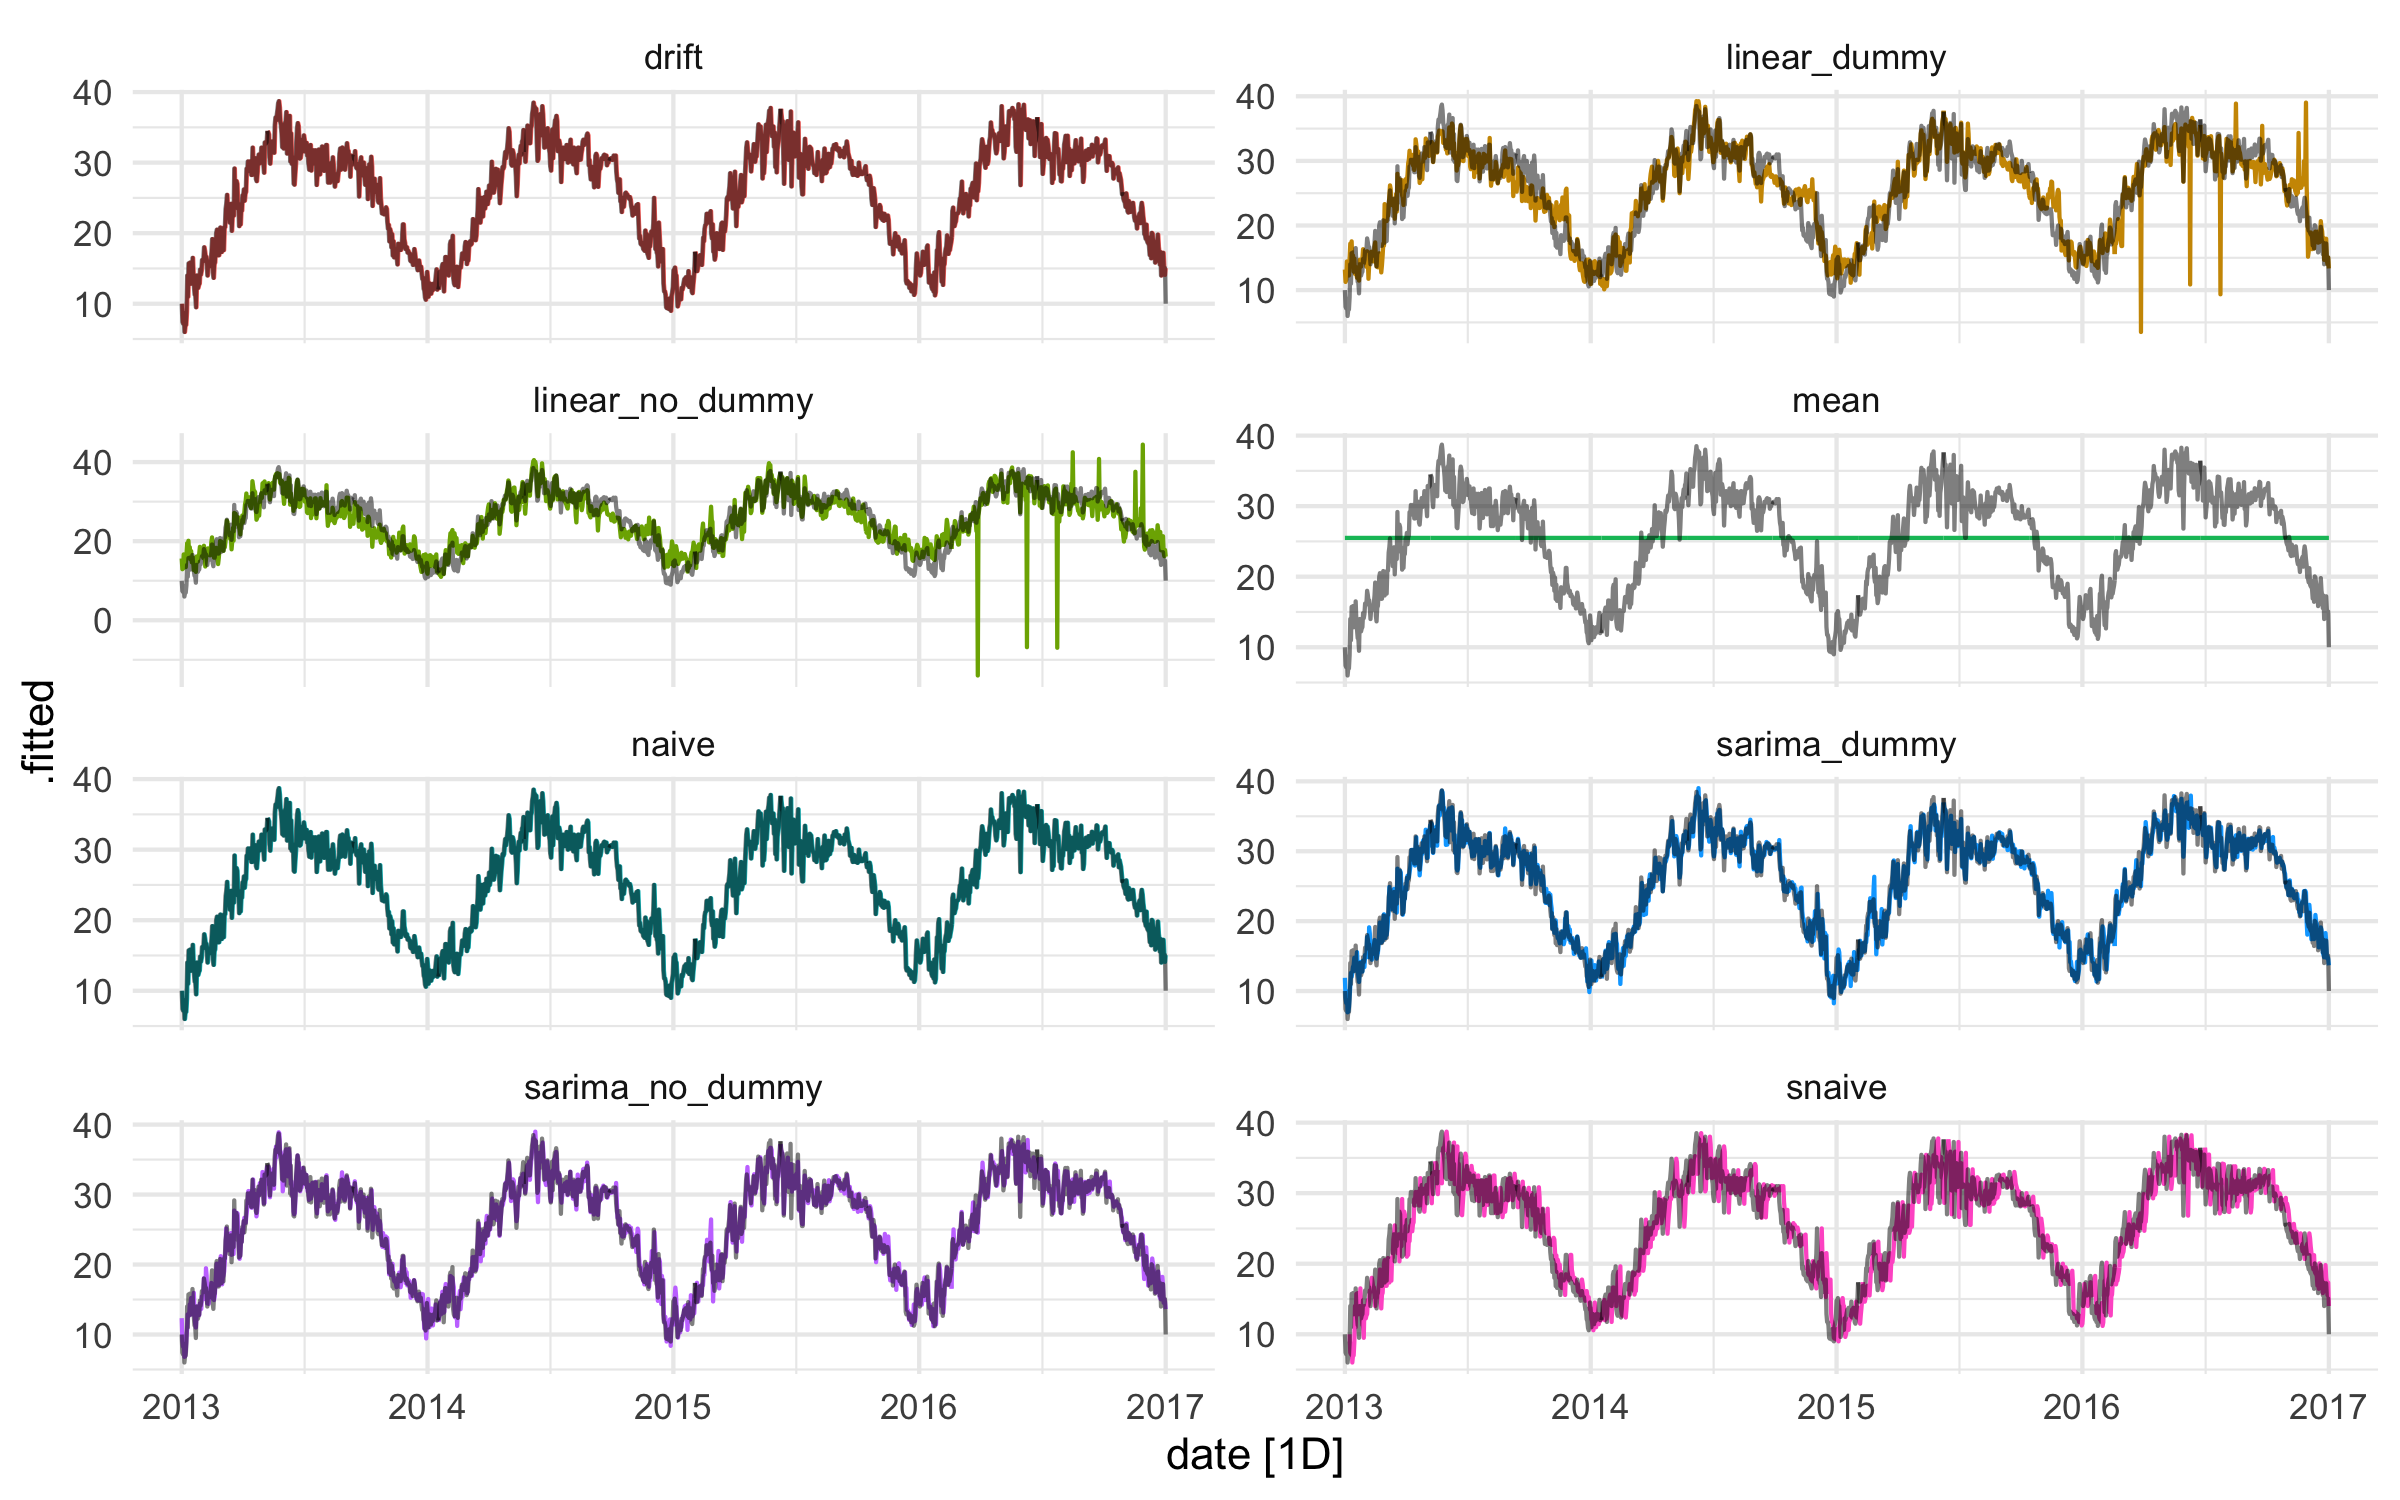
\includegraphics[width=.8\textwidth]{images/fitted_values_all_models.png}
    \caption{\small \textit{Fitted values and the true values on training data}}
    \label{fig:figure1}
\end{figure}

\begin{figure}[!h]
    \centering
    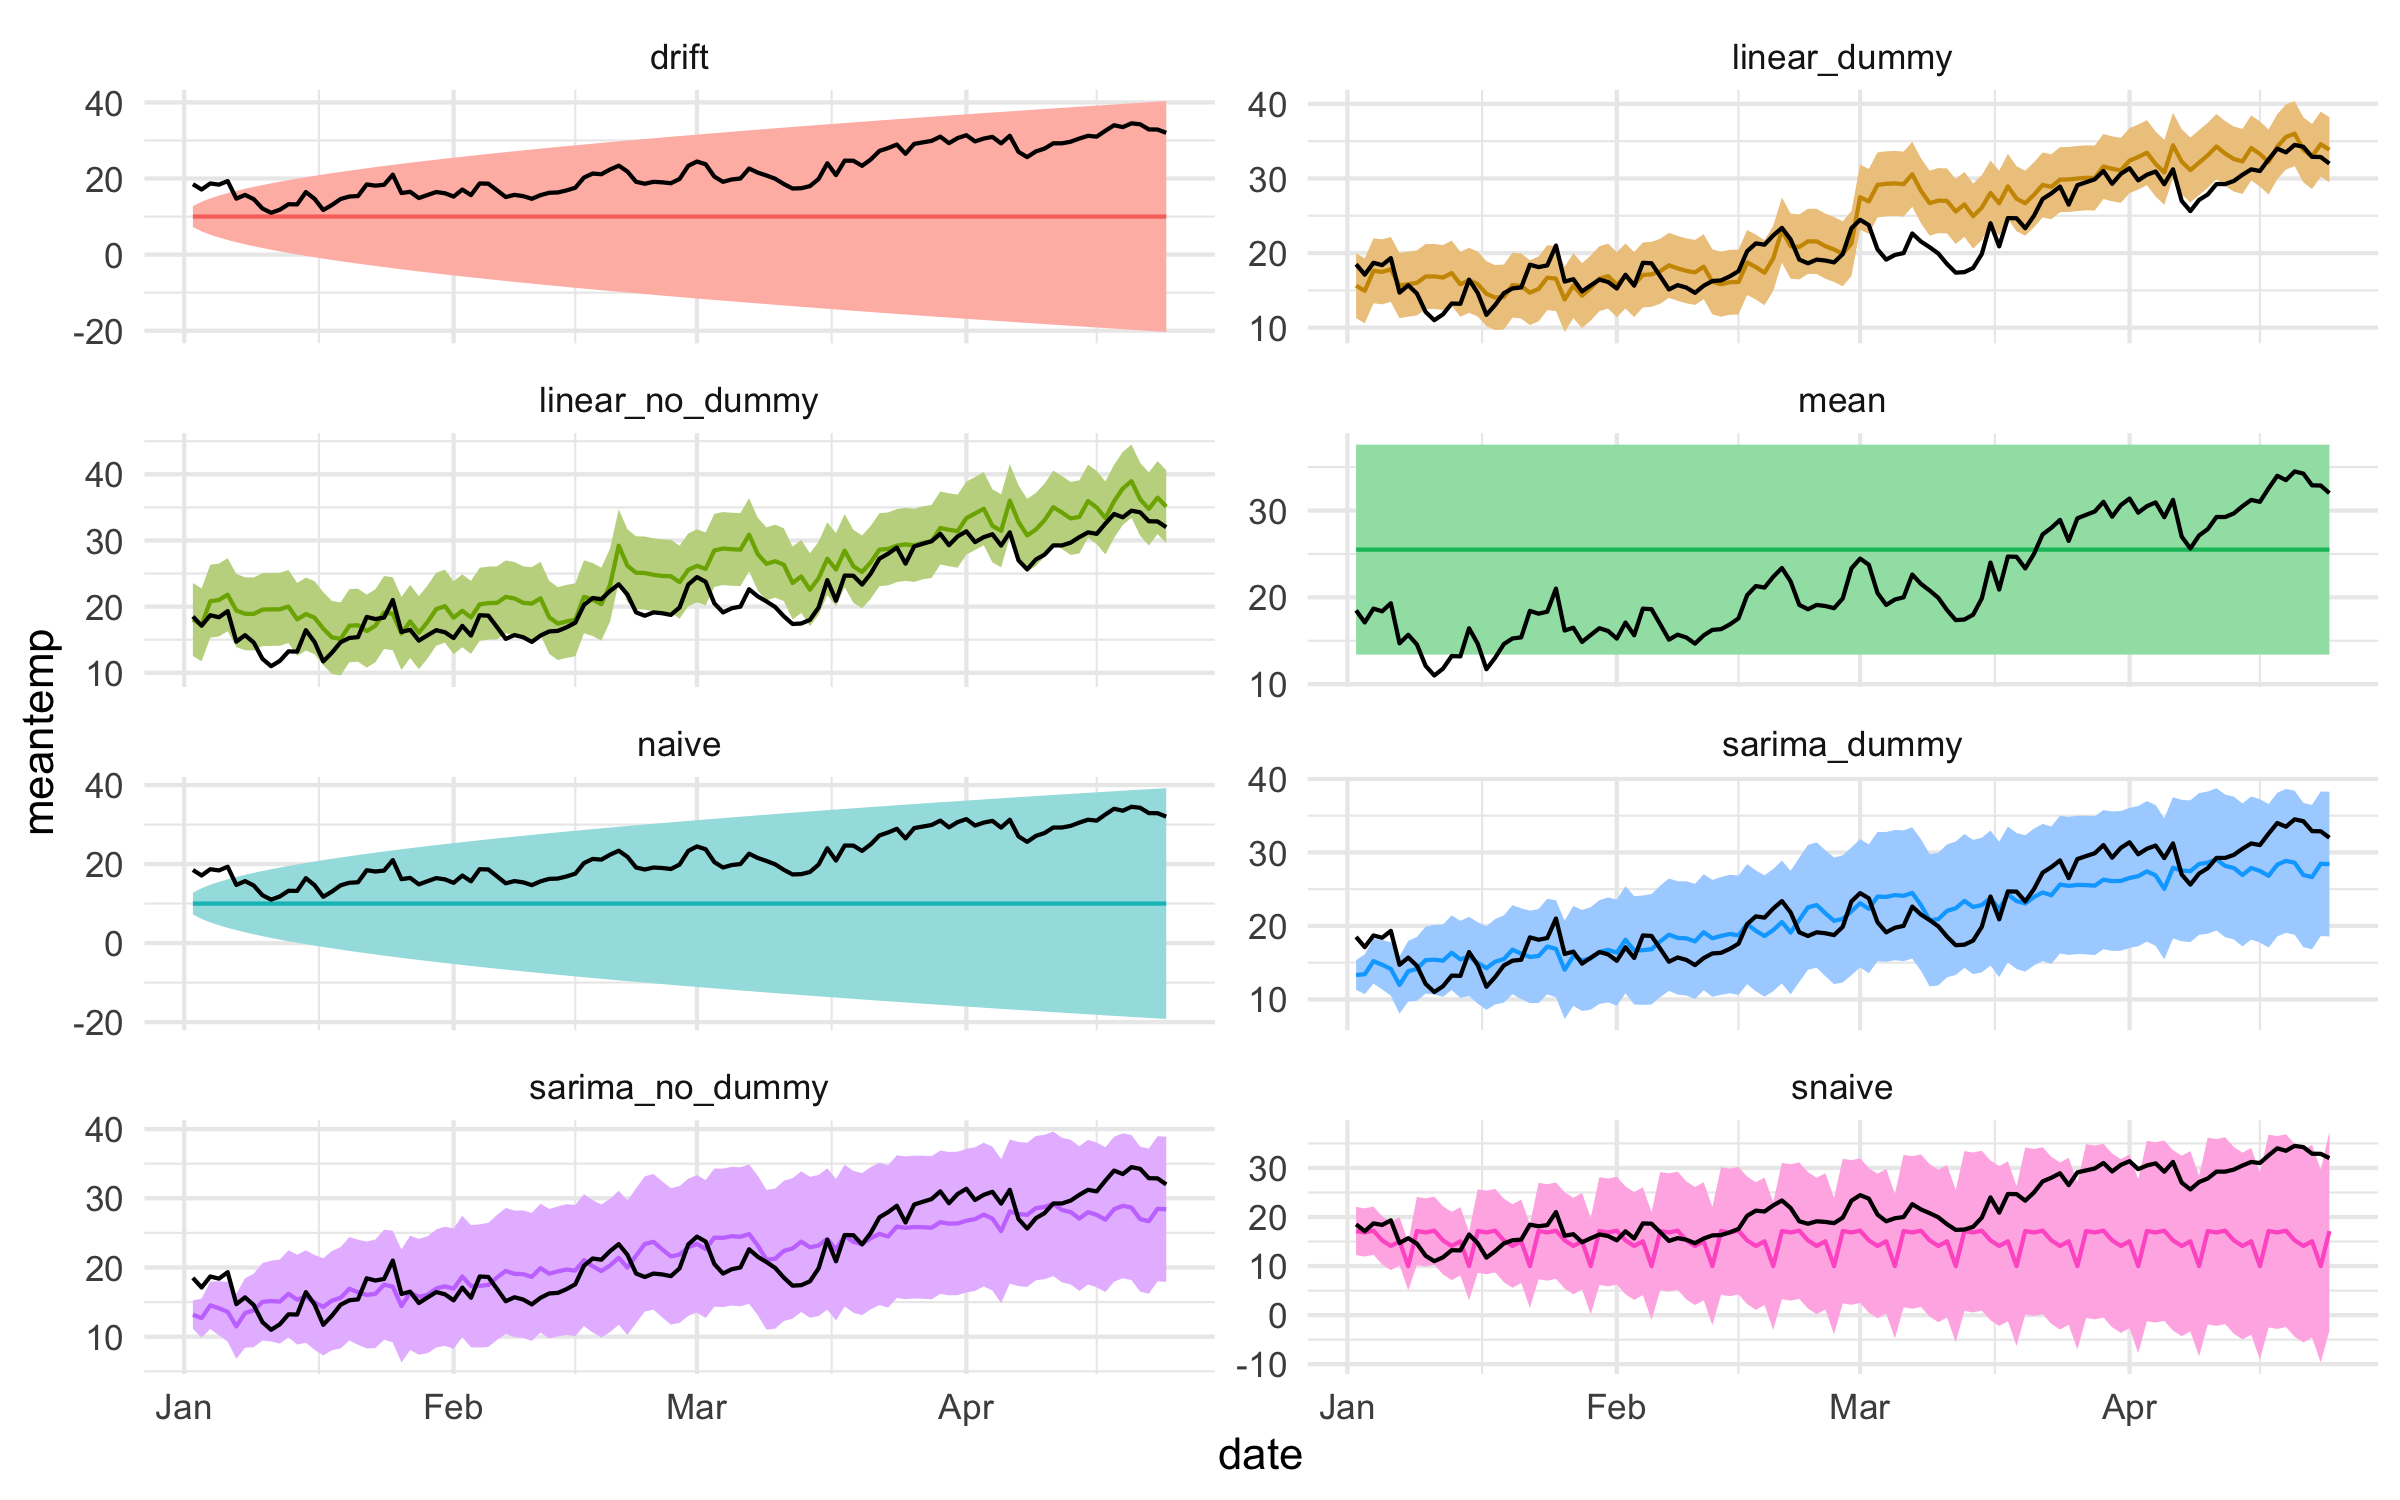
\includegraphics[width=.8\textwidth]{images/forecasts_CI90.png}
    \caption{\small \textit{Forecasts with 90\% confidence interval of all models}}
    \label{fig:figure1}
\end{figure}

\begin{figure}[!h]
    \centering
    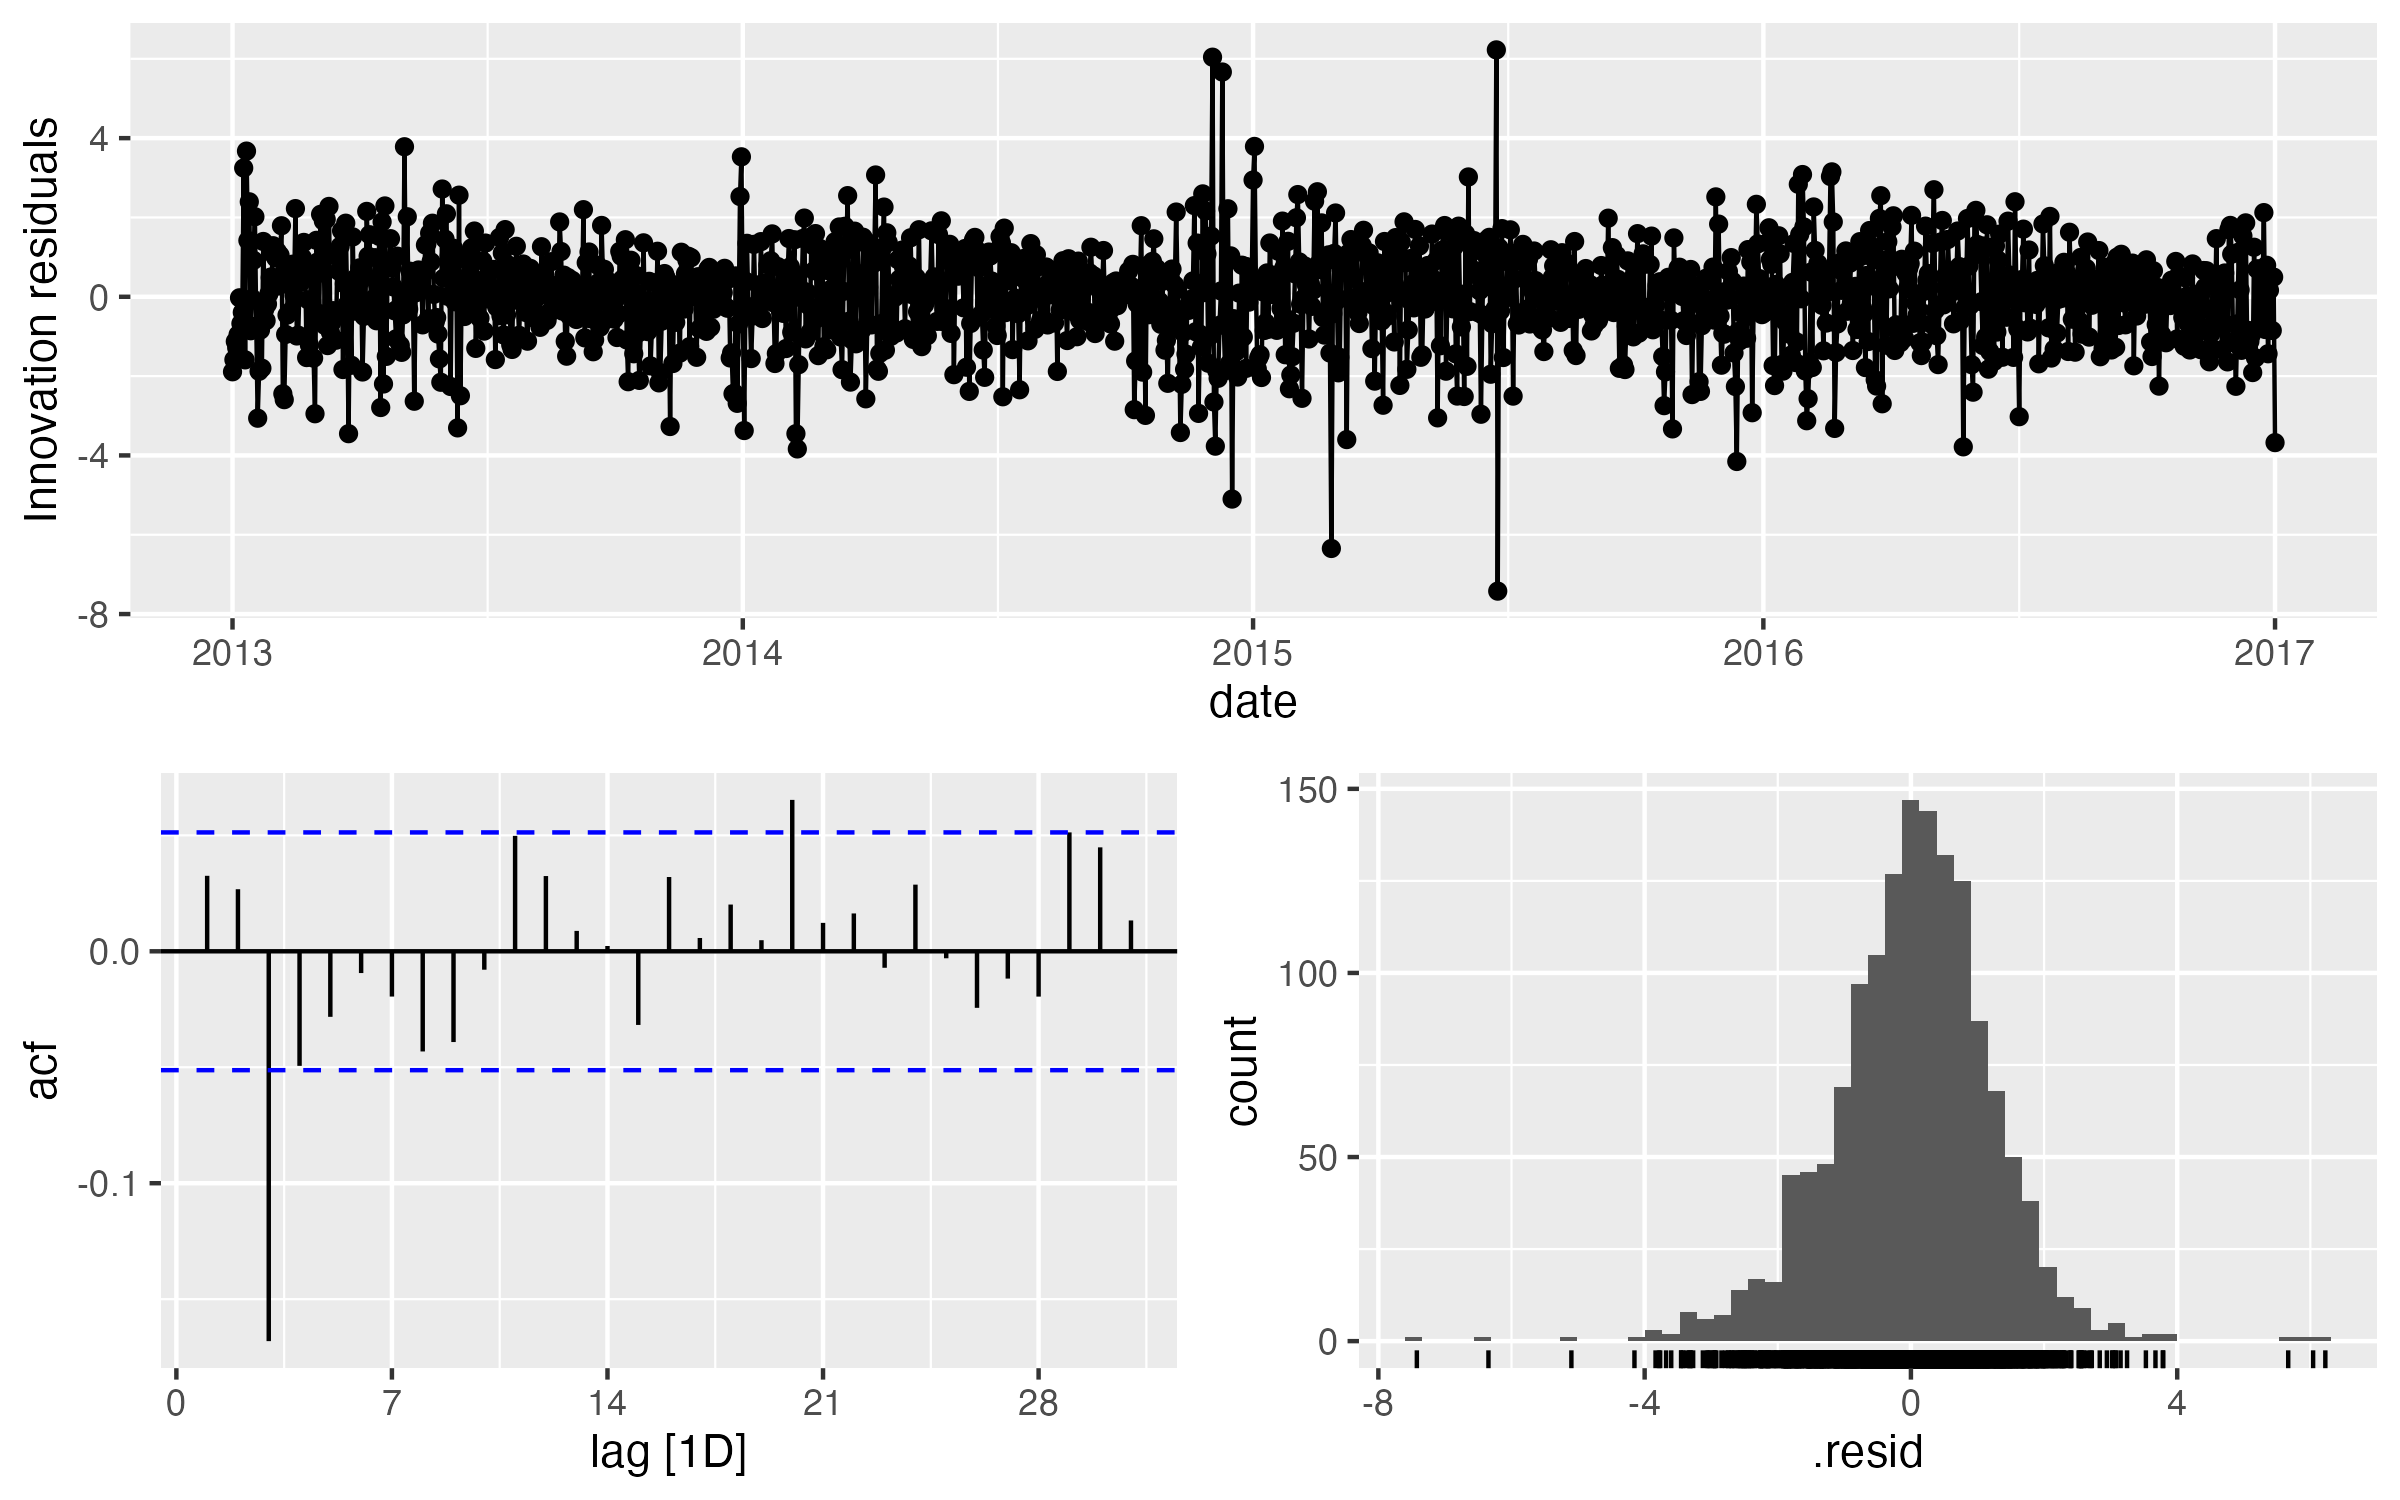
\includegraphics[width=.8\textwidth]{images/best_model_resid_diagnostic.png}
    \caption{\small \textit{Residual diagnostic plot for SARIMA with dummy variables}}
    \label{fig:figure1}
\end{figure}

\begin{figure}[!h]
    \centering
    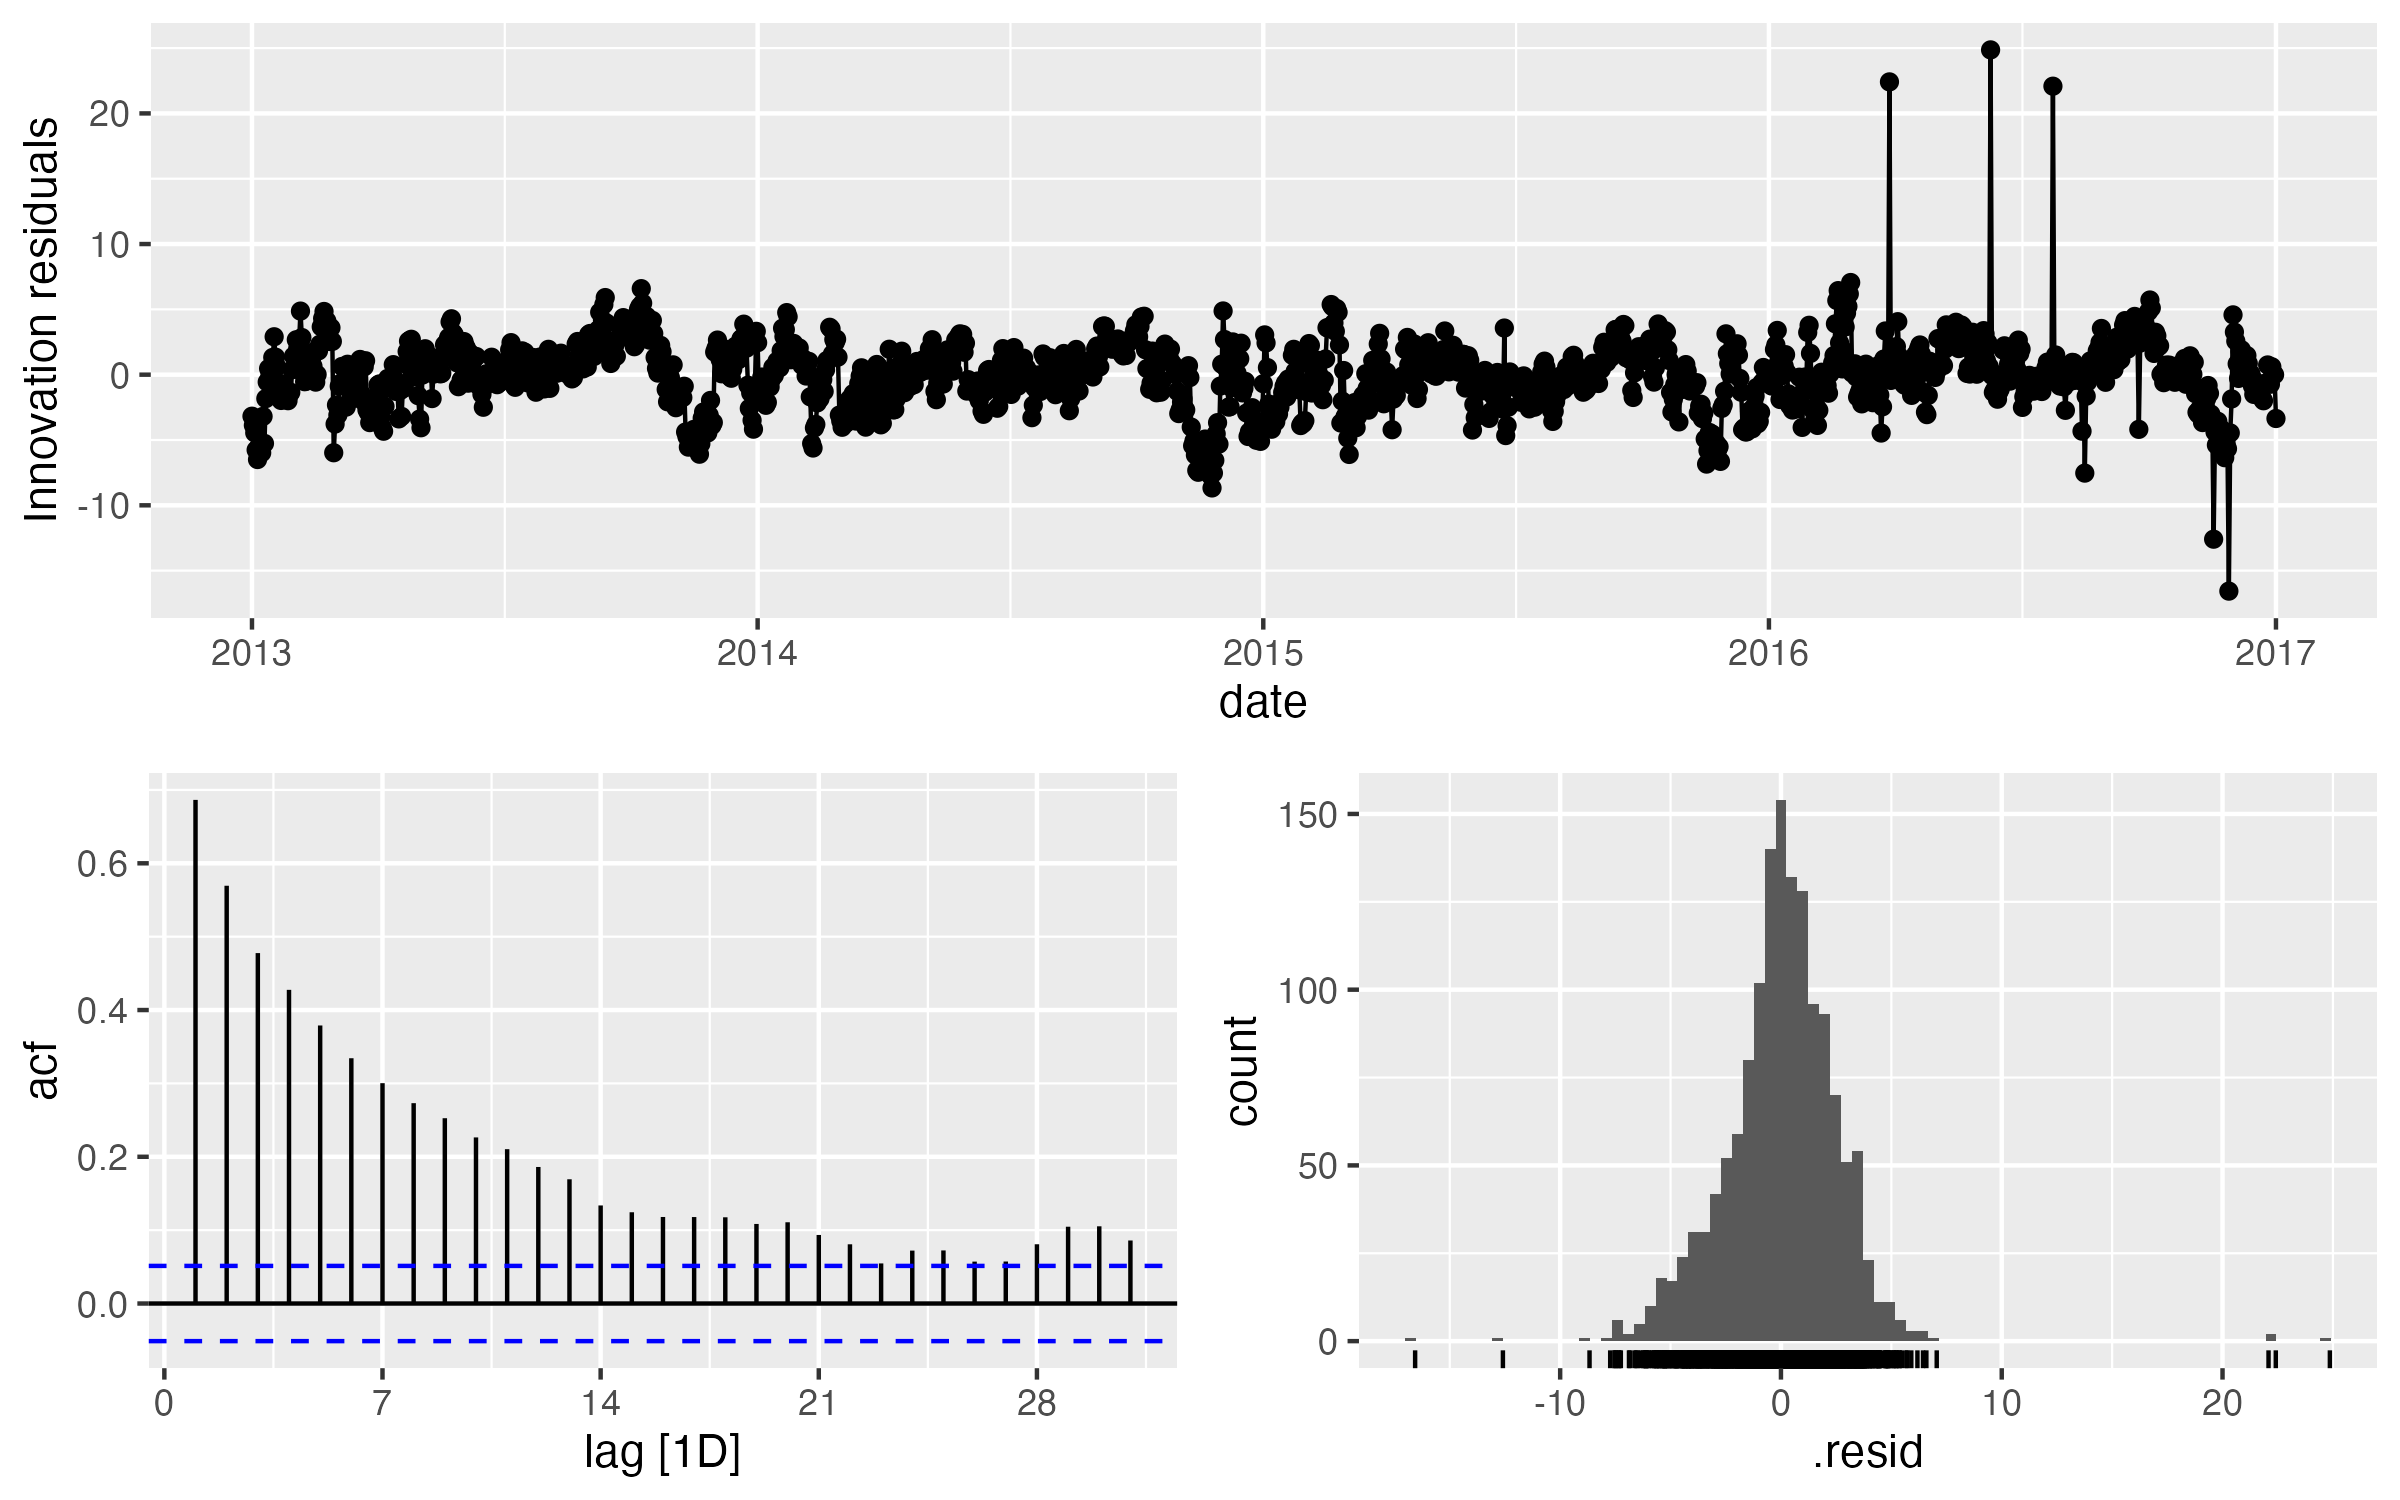
\includegraphics[width=.8\textwidth]{images/linear_dummy_model_resid_diagnostic.png}
    \caption{\small \textit{Residual diagnostic plot for standard linear model with dummy variables}}
    \label{fig:figure1}
\end{figure}







\clearpage
\subsection{Tables}

\begin{table}[!h]
    \centering
    \caption{\small \textit{Mean features for different seasons}}
    \centering
    \begin{tabular}[t]{lrrrr}
    \toprule
    season & mean\_temp & mean\_pressure & mean\_w\_speed & mean\_humidity\\
    \midrule
    Autumn & 26.0792 & 1009.7134 & 5.4029 & 60.8571\\
    Spring & 28.5264 & 1007.4021 & 8.4979 & 45.2249\\
    Summer & 31.7559 & 999.5255 & 7.8920 & 64.0544\\
    Winter & 15.4633 & 1016.7316 & 5.3775 & 73.1533\\
    \bottomrule
    \end{tabular}
\end{table}

\begin{table}[!h]
    \centering
    \caption{\small \textit{Models built in this report}}
    \label{tab:model_classification}
    \begin{tabular}{|c|c|c|}
    \hline
    \textbf{Basic Model} & \textbf{With Dummy}    & \textbf{Without Dummy}   \\ \hline
    Drift                & Linear Dummy           & Linear No Dummy          \\ 
    Mean                 & Sarima Dummy           & Sarima No Dummy          \\ 
    Naive                &                        &                          \\ 
    SNaive               &                        &                          \\ \hline
    \end{tabular}
\end{table}


\begin{table}[!h]
    \centering
    \caption{\small \textit{Performance of models}}
    \centering
    \begin{tabular}[t]{lrrrrrr}
    \toprule
    .model & adj\_r\_squared & sigma2 & log\_lik & AICc & BIC & df.residual\\
    \midrule
    linear\_no\_dummy & 0.7928 & 11.1880 & -3837.231 & 3537.543 & 3569.210 & 1457\\
    linear\_dummy & 0.8709 & 6.9699 & -3489.786 & 2848.720 & 2896.184 & 1454\\
    naive & NA & 2.7938 & NA & NA & NA & NA\\
    snaive & NA & 8.9231 & NA & NA & NA & NA\\
    drift & NA & 2.7938 & NA & NA & NA & NA\\
    \addlinespace
    mean & NA & 53.9946 & NA & NA & NA & NA\\
    sarima\_dummy & NA & 1.5048 & -2369.349 & 4762.914 & 4826.149 & NA\\
    sarima\_no\_dummy & NA & 1.5381 & -2387.348 & 4790.795 & 4832.996 & NA\\
    \bottomrule
    \end{tabular}
\end{table}

\begin{table}[!h]
    \centering
    \caption{\small \textit{Comparisions of criteria for forecasting}}
    \centering
    \begin{tabular}[t]{lrrrrr}
    \toprule
    .model & RMSE & MAE & MPE & MAPE & ACF1\\
    \midrule
    sarima\_dummy & 3.0829 & 2.6184 & -0.0790 & 12.4737 & 0.8543\\
    sarima\_no\_dummy & 3.1777 & 2.7123 & -1.6050 & 13.1857 & 0.8641\\
    linear\_dummy & 3.6619 & 2.7407 & -9.3986 & 13.7899 & 0.8673\\
    linear\_no\_dummy & 4.2402 & 3.5275 & -17.8293 & 18.4615 & 0.7798\\
    mean & 7.3533 & 6.5861 & -27.4088 & 36.5698 & 0.9525\\
    \addlinespace
    snaive & 9.5219 & 7.3749 & 24.3618 & 29.8995 & 0.8207\\
    drift & 13.3623 & 11.7644 & 50.0270 & 50.0270 & 0.9525\\
    naive & 13.3623 & 11.7644 & 50.0270 & 50.0270 & 0.9525\\
    \bottomrule
    \end{tabular}
\end{table}

\begin{table}[!h]
    \centering
    \caption{\small \textit{Tests on residuals from models' fitted values}}
    \centering
    \begin{tabular}[t]{lrrrrrr}
    \toprule
    .model & kpss\_stat & kpss\_pvalue & bp\_stat & bp\_pvalue & lb\_stat & lb\_pvalue\\
    \midrule
    drift & 0.1668 & 0.1000 & 37.3479 & 0.0000 & 37.4246 & 0.0000\\
    linear\_dummy & 0.1640 & 0.1000 & 688.8547 & 0.0000 & 690.2692 & 0.0000\\
    linear\_no\_dummy & 0.1899 & 0.1000 & 473.1878 & 0.0000 & 474.1595 & 0.0000\\
    mean & 0.5774 & 0.0247 & 1378.7251 & 0.0000 & 1381.5562 & 0.0000\\
    naive & 0.1668 & 0.1000 & 37.3479 & 0.0000 & 37.4246 & 0.0000\\
    \addlinespace
    sarima\_dummy & 0.1538 & 0.1000 & 1.5492 & 0.2133 & 1.5524 & 0.2128\\
    sarima\_no\_dummy & 0.0711 & 0.1000 & 0.0115 & 0.9145 & 0.0116 & 0.9144\\
    snaive & 0.2894 & 0.1000 & 672.6339 & 0.0000 & 674.0218 & 0.0000\\
    \bottomrule
    \end{tabular}
\end{table}

\begin{table}[h]
    \centering
    \caption{\small \textit{Specific coefficients and statistics}}
    \centering
    \begin{tabular}[t]{llrrrr}
    \toprule
    .model & term & estimate & std.error & statistic & p.value\\
    \midrule
    linear\_no\_dummy & (Intercept) & 700.3787 & 11.8561 & 59.0733 & 0.0000\\
    linear\_no\_dummy & humidity & -0.1567 & 0.0058 & -27.0830 & 0.0000\\
    linear\_no\_dummy & wind\_speed & -0.0409 & 0.0211 & -1.9380 & 0.0528\\
    linear\_no\_dummy & meanpressure & -0.6612 & 0.0118 & -56.0071 & 0.0000\\
    linear\_no\_dummy & time & 0.0021 & 0.0002 & 10.3031 & 0.0000\\
    \addlinespace
    linear\_dummy & (Intercept) & 419.8945 & 14.5850 & 28.7894 & 0.0000\\
    linear\_dummy & humidity & -0.1399 & 0.0056 & -24.8596 & 0.0000\\
    linear\_dummy & wind\_speed & -0.0106 & 0.0169 & -0.6284 & 0.5298\\
    linear\_dummy & meanpressure & -0.3888 & 0.0144 & -26.9365 & 0.0000\\
    linear\_dummy & time & 0.0017 & 0.0002 & 10.1253 & 0.0000\\
    \addlinespace
    linear\_dummy & season\_Autumn & 5.9208 & 0.2251 & 26.3036 & 0.0000\\
    linear\_dummy & season\_Spring & 5.6261 & 0.2601 & 21.6269 & 0.0000\\
    linear\_dummy & season\_Summer & 8.2651 & 0.3086 & 26.7856 & 0.0000\\
    drift & b & 0.0000 & 0.0437 & 0.0000 & 1.0000\\
    sarima\_dummy & ar1 & 0.9898 & 0.0041 & 242.1087 & 0.0000\\
    \addlinespace
    sarima\_dummy & ma1 & -0.0953 & 0.0298 & -3.2015 & 0.0014\\
    sarima\_dummy & ma2 & -0.1798 & 0.0300 & -5.9982 & 0.0000\\
    sarima\_dummy & humidity & -0.1363 & 0.0042 & -32.4098 & 0.0000\\
    sarima\_dummy & wind\_speed & -0.0291 & 0.0072 & -4.0637 & 0.0001\\
    sarima\_dummy & meanpressure & -0.0322 & 0.0076 & -4.2461 & 0.0000\\
    \addlinespace
    sarima\_dummy & time & 0.0021 & 0.0045 & 0.4730 & 0.6363\\
    sarima\_dummy & season\_Autumn & 0.2608 & 0.5227 & 0.4990 & 0.6179\\
    sarima\_dummy & season\_Spring & 0.5930 & 0.5235 & 1.1326 & 0.2576\\
    sarima\_dummy & season\_Summer & 0.4116 & 0.6098 & 0.6751 & 0.4997\\
    sarima\_dummy & intercept & 63.9278 & 8.5701 & 7.4594 & 0.0000\\
    \addlinespace
    sarima\_no\_dummy & ar1 & 0.9821 & 0.0054 & 180.2766 & 0.0000\\
    sarima\_no\_dummy & ma1 & -0.0234 & 0.0329 & -0.7128 & 0.4761\\
    sarima\_no\_dummy & humidity & -0.1355 & 0.0042 & -32.3052 & 0.0000\\
    sarima\_no\_dummy & wind\_speed & -0.0305 & 0.0070 & -4.3544 & 0.0000\\
    sarima\_no\_dummy & meanpressure & -0.0321 & 0.0075 & -4.2714 & 0.0000\\
    \addlinespace
    sarima\_no\_dummy & time & -0.0001 & 0.0039 & -0.0339 & 0.9730\\
    sarima\_no\_dummy & intercept & 66.1415 & 8.2258 & 8.0408 & 0.0000\\
    \bottomrule
    \end{tabular}
\end{table}





\end{document}